\documentclass[a4paper]{scrbook}
\usepackage{lmodern}
\usepackage{amssymb,amsmath}
\usepackage{ifxetex,ifluatex}
\usepackage{fixltx2e} % provides \textsubscript
\ifnum 0\ifxetex 1\fi\ifluatex 1\fi=0 % if pdftex
  \usepackage[T1]{fontenc}
  \usepackage[utf8]{inputenc}
\else % if luatex or xelatex
  \ifxetex
    \usepackage{mathspec}
  \else
    \usepackage{fontspec}
  \fi
  \defaultfontfeatures{Ligatures=TeX,Scale=MatchLowercase}
\fi
% use upquote if available, for straight quotes in verbatim environments
\IfFileExists{upquote.sty}{\usepackage{upquote}}{}
% use microtype if available
\IfFileExists{microtype.sty}{%
\usepackage{microtype}
\UseMicrotypeSet[protrusion]{basicmath} % disable protrusion for tt fonts
}{}
\usepackage[unicode=true]{hyperref}
\hypersetup{
            pdftitle={経済動学 (線形モデル)},
            pdfauthor={佐藤 健治},
            pdfborder={0 0 0},
            breaklinks=true}
\urlstyle{same}  % don't use monospace font for urls
\usepackage{natbib}
\bibliographystyle{apalike}
\usepackage{color}
\usepackage{fancyvrb}
\newcommand{\VerbBar}{|}
\newcommand{\VERB}{\Verb[commandchars=\\\{\}]}
\DefineVerbatimEnvironment{Highlighting}{Verbatim}{commandchars=\\\{\}}
% Add ',fontsize=\small' for more characters per line
\usepackage{framed}
\definecolor{shadecolor}{RGB}{248,248,248}
\newenvironment{Shaded}{\begin{snugshade}}{\end{snugshade}}
\newcommand{\KeywordTok}[1]{\textcolor[rgb]{0.13,0.29,0.53}{\textbf{{#1}}}}
\newcommand{\DataTypeTok}[1]{\textcolor[rgb]{0.13,0.29,0.53}{{#1}}}
\newcommand{\DecValTok}[1]{\textcolor[rgb]{0.00,0.00,0.81}{{#1}}}
\newcommand{\BaseNTok}[1]{\textcolor[rgb]{0.00,0.00,0.81}{{#1}}}
\newcommand{\FloatTok}[1]{\textcolor[rgb]{0.00,0.00,0.81}{{#1}}}
\newcommand{\ConstantTok}[1]{\textcolor[rgb]{0.00,0.00,0.00}{{#1}}}
\newcommand{\CharTok}[1]{\textcolor[rgb]{0.31,0.60,0.02}{{#1}}}
\newcommand{\SpecialCharTok}[1]{\textcolor[rgb]{0.00,0.00,0.00}{{#1}}}
\newcommand{\StringTok}[1]{\textcolor[rgb]{0.31,0.60,0.02}{{#1}}}
\newcommand{\VerbatimStringTok}[1]{\textcolor[rgb]{0.31,0.60,0.02}{{#1}}}
\newcommand{\SpecialStringTok}[1]{\textcolor[rgb]{0.31,0.60,0.02}{{#1}}}
\newcommand{\ImportTok}[1]{{#1}}
\newcommand{\CommentTok}[1]{\textcolor[rgb]{0.56,0.35,0.01}{\textit{{#1}}}}
\newcommand{\DocumentationTok}[1]{\textcolor[rgb]{0.56,0.35,0.01}{\textbf{\textit{{#1}}}}}
\newcommand{\AnnotationTok}[1]{\textcolor[rgb]{0.56,0.35,0.01}{\textbf{\textit{{#1}}}}}
\newcommand{\CommentVarTok}[1]{\textcolor[rgb]{0.56,0.35,0.01}{\textbf{\textit{{#1}}}}}
\newcommand{\OtherTok}[1]{\textcolor[rgb]{0.56,0.35,0.01}{{#1}}}
\newcommand{\FunctionTok}[1]{\textcolor[rgb]{0.00,0.00,0.00}{{#1}}}
\newcommand{\VariableTok}[1]{\textcolor[rgb]{0.00,0.00,0.00}{{#1}}}
\newcommand{\ControlFlowTok}[1]{\textcolor[rgb]{0.13,0.29,0.53}{\textbf{{#1}}}}
\newcommand{\OperatorTok}[1]{\textcolor[rgb]{0.81,0.36,0.00}{\textbf{{#1}}}}
\newcommand{\BuiltInTok}[1]{{#1}}
\newcommand{\ExtensionTok}[1]{{#1}}
\newcommand{\PreprocessorTok}[1]{\textcolor[rgb]{0.56,0.35,0.01}{\textit{{#1}}}}
\newcommand{\AttributeTok}[1]{\textcolor[rgb]{0.77,0.63,0.00}{{#1}}}
\newcommand{\RegionMarkerTok}[1]{{#1}}
\newcommand{\InformationTok}[1]{\textcolor[rgb]{0.56,0.35,0.01}{\textbf{\textit{{#1}}}}}
\newcommand{\WarningTok}[1]{\textcolor[rgb]{0.56,0.35,0.01}{\textbf{\textit{{#1}}}}}
\newcommand{\AlertTok}[1]{\textcolor[rgb]{0.94,0.16,0.16}{{#1}}}
\newcommand{\ErrorTok}[1]{\textcolor[rgb]{0.64,0.00,0.00}{\textbf{{#1}}}}
\newcommand{\NormalTok}[1]{{#1}}
\usepackage{longtable,booktabs}
\usepackage{graphicx,grffile}
\makeatletter
\def\maxwidth{\ifdim\Gin@nat@width>\linewidth\linewidth\else\Gin@nat@width\fi}
\def\maxheight{\ifdim\Gin@nat@height>\textheight\textheight\else\Gin@nat@height\fi}
\makeatother
% Scale images if necessary, so that they will not overflow the page
% margins by default, and it is still possible to overwrite the defaults
% using explicit options in \includegraphics[width, height, ...]{}
\setkeys{Gin}{width=\maxwidth,height=\maxheight,keepaspectratio}
\IfFileExists{parskip.sty}{%
\usepackage{parskip}
}{% else
\setlength{\parindent}{0pt}
\setlength{\parskip}{6pt plus 2pt minus 1pt}
}
\setlength{\emergencystretch}{3em}  % prevent overfull lines
\providecommand{\tightlist}{%
  \setlength{\itemsep}{0pt}\setlength{\parskip}{0pt}}
\setcounter{secnumdepth}{5}
% Redefines (sub)paragraphs to behave more like sections
\ifx\paragraph\undefined\else
\let\oldparagraph\paragraph
\renewcommand{\paragraph}[1]{\oldparagraph{#1}\mbox{}}
\fi
\ifx\subparagraph\undefined\else
\let\oldsubparagraph\subparagraph
\renewcommand{\subparagraph}[1]{\oldsubparagraph{#1}\mbox{}}
\fi
\usepackage[hiragino-pron]{luatexja-preset}
\usepackage{amsthm}

\theoremstyle{definition}
\newtheorem{theorem}{定理}[chapter]
\newtheorem{proposition}{命題}[chapter]
\newtheorem{definition}{定義}[chapter]
\newtheorem{lemma}{補題}[chapter]
\newtheorem{fact}{事実}[chapter]
\newtheorem{exercise}{練習問題}[chapter]

\makeatletter
\def\thm@space@setup{%
  \thm@preskip=8pt plus 2pt minus 4pt
  \thm@postskip=\thm@preskip
}
\makeatother

\usepackage[onehalfspacing]{setspace}
\setlength{\abovedisplayskip}{1pt}
\setlength{\belowdisplayskip}{1pt}

\title{経済動学 (線形モデル)}
\author{佐藤 健治}
\date{2017-02-04}

\let\BeginKnitrBlock\begin \let\EndKnitrBlock\end
\begin{document}
\maketitle

{
\setcounter{tocdepth}{1}
\tableofcontents
}
\chapter*{序文}
\addcontentsline{toc}{chapter}{序文}

このノートは, 神戸大学大学院経済学研究科で2016年度,
2017年度の第1クォーターに実施した講義に基づいている. マクロ経済学,
マクロ計量経済学,
および数理経済学を専攻しようとする院生を読者として想定しているが,
数学的な議論が苦にならなければ学部生にとっても有益なものと思われる.
線形代数学, 動的システム理論, 力学系の初歩的な概念からはじめて,
できるかぎり自己完結的なものとなるように心がけたので,
マクロ経済学に特化した「経済数学」という使いかたもできると思う.

この講義では, 線形合理的期待モデルの分析を中心的な課題としている.
次の3つを中心的な課題としている.

\begin{itemize}
\tightlist
\item
  線形合理的期待モデルの理論分析
\item
  その計算機シミュレーション
\item
  マルコフスイッチング合理的期待モデルの紹介
\end{itemize}

マクロ数量分析の標準的なツールである Dynare を自分で使ったり,
論文で名前を見たことがある学生も多いと思う. 一方で,
その裏側でどのような計算が行われているかを知らないという学生も多いのではないかと思う.
理論に無関心でもおおよそ問題が起こらないのは, ひとえに Dynare
が優れたインターフェイスを備えたアプリケーションであるということに外ならないのだが,
そのブラックボックスを開けて理論を理解しようというのがこの講義の第1の課題である.

第2の課題は,
読者にコンピュータシミュレーションの基礎的な手法を身につけてもらうことである.
線形合理的期待モデルは近年のマクロ経済の数量分析に大きな役割を果たしているから,
各自の研究プロジェクトに大いに役に立つものと信じている.
数学もプログラミングも自分の手を動かし, 頭を悩ませなければ習熟できない.
理論とその実装を行き来しながら総合的な問題解決能力を養ってほしい.
この講義では, 主に R言語を用いる.\footnote{R
  (\url{https://www.r-project.org/}) と RStudio
  (\url{https://www.rstudio.com/}) の最新版を各自インストールしてほしい.
  R言語を選んだ理由は,
  計量経済学の学習のために利用したことのある学生が多いだろう考えたからであり,
  R がシミュレーションのために最適であるとは考えていない.
  大変人気のあるプログラミング言語・環境であるから一度は学んでおいて損はないと思う.}

最後に,
近年盛んに研究されているマルコフスイッチング合理的期待モデルという非線形モデルを紹介する.
線形モデルのように, (ある種の)
安定性・不安定性に関する必要十分条件が得られるという特徴があり,
理論的に扱いやすい.
金融政策ルールに関するテイラーの条件を緩和できることが知られており,
理論・実証の両面から盛んに研究が進んでいる分野である.

\section*{構成}
\addcontentsline{toc}{section}{構成}

\begin{itemize}
\tightlist
\item
  第\ref{intro}章: はじめに
\item
  第\ref{complexnumbers}章: 複素数
\item
  第\ref{matrix}章: 行列理論
\item
  第?章: 標準形と線形システム
\item
  第?章: \(\det A \neq 0\)
\item
  第?章: 一般の \(A\)
\end{itemize}

\section*{謝辞}
\addcontentsline{toc}{section}{謝辞}

コロンビア大学の安東宇さんから有益なコメントをいくつかいただいた.

\chapter{はじめに}\label{intro}

\section{目標とするモデル}

この講義では, 次の形の動的システムを考察する.

\[
\begin{equation}
  A\mathbb{E}_{t}x_{t+1}=Bx_{t}+Cz_{t} \label{eq:lre}
\end{equation}
\]

\(x_t\) は内生変数のベクトル, \(z_t\) は外生変数. \(A\), \(B\), \(C\)
は適切なサイズの行列である. \(\mathbb E_t\) は条件付き期待値.
大ざっぱに言えば,
行列積と足し算だけからなるシステムを線形システムという. 上の線形方程式を

\begin{equation} 
  Bx_{t} = A\mathbb{E}_{t}x_{t+1} - Cz_{t} \label{eq:lre2}
\end{equation}

と書き換えると,
\textbf{今期の経済変数は将来に対する期待によって定まっている}と読むことができる.
\eqref{eq:lre} や \eqref{eq:lre2} のようなシステムを
\textbf{線形合理的期待モデル (linear rational expectations model)}
という.

通常, 経済モデルは非線形システム
(線形でないシステムをすべて非線形システムという)
によって記述されることが多いのだが, 非確率的な平衡点
\(x^* = x_t = x_{t+1}\), \(z_t = 0\) (\(t > 0\))
の周りに分析を限定すれば,
線形システムによってよく近似されることが知られている.\footnote{Hartman-Grobman
  の定理.}

線形システムの分析は係数行列 (上記の \(A\), \(B\), \(C\))
の分析に落とし込むことができるため, 理論的にも数値的にも大変扱いやすい.
したがって,
これから我々が学ぶ分析手法は\textbf{平衡状態にある経済に対して小さなショックが加わったときに,
経済変数がどのような経時的変化を示すかを分析するための第一歩}である.
実際には,
線形近似のみから数量的なインプリケーションを導くことは困難であるり,
有用な分析を行うためには高次の近似手法を学ぶ必要がある. しかし,
線形理論を理解することなく非線形理論を理解することはできない.
一歩一歩着実に進んでいこう.

\section{最初のモデル}

実は確率的な要因がなくなったとしても分析の基本的な方針は変わらない.
すなわち, 非確率的 (決定論的) なシステム

\begin{equation}
  Ax_{t+1} = Bx_t + Cz_t \label{eq:lsys}
\end{equation}

を分析する手法を確立すれば, \eqref{eq:lre}
の分析・シミュレーションができる. まずは \eqref{eq:lsys}
の分析について述べたのち,
確率的な要因を導入するというステップで理論分析を進める.

上記の \eqref{eq:lsys} の形のシステムは,
制御理論の分野ではデスクリプタシステム (descriptor system),
あるいは陰的システム (implicit system) として知られている.
制御理論における前提とやや異なる部分もあるにはあるが,
基本的な方針を概ね共有している. この分野で研究を進めようという人は,
同じ概念が異なる分野で異なる名前で利用されていることを知っておく方がよいだろう.

\section{プログラミング環境 RStudio}\label{-rstudio}

前述のような線形モデルは (広く普及している C, Fortran
のルーチンのおかげで) 大抵のプログラミング言語で解くことができる. 本書で
R を使用するのは,
想定する読者層がもっとも接近しやすい言語であろうと考えたからである.
計量経済学の学習は Stata を使い, マクロ経済学では Matlab,
数理経済学の授業では Python というようなことにもなりがちだが,
プログラミングの初級者は1つの言語に深く習熟するようにした方がよい.
将来的に他の言語に移るとしても,
広く浅く学んだ人よりも深く狭く学んだ人の方が, 速く学ぶ.

R は計量経済学のツールとしてもとても優秀で,
しかも多くのユーザーコミュニティがある. データ収集, 図示, モデリング,
ドキュメント作成のすべての工程をRとRStudio で実行することができる.
RStudio に触れる機会を増やすために, すべてのレポートを RStudio
で作成するように気持ちを切り替えてみよう. RMarkdown という書式で書き,
それをコンパイルする. knitr や pandoc がスムーズに仕事をこなしてくれる.
PDF に変換するには texlive をインストールする. サイズは大きいが簡単だ.
数式を入力するには LaTeX の構文を覚える必要があるが,
大学院にいる以上いずれ必要になる技術だ. 今やって損はない. RMarkdown は
LaTeX そのものと比べると概ね自然に書くことができるし, 何よりも R
のコードや計算結果, グラフを文章内に埋め込むのが非常に簡単だ. ところで,
本書も RStudio で書いている. いくつかの RMarkdown ファイル,
設定ファイルを bookdown というパッケージがうまく処理してくれる.

R に十分習熟し,
プロファイリングの努力も虚しく計算速度に限界を感じることがあるかもしれない.
そうなった C++ を少し学べばよい. 重い処理だけを扱う C++
のコードを用意し, RCpp パケージを使って呼び出すことができる.
そのような願望が現れるころには計算機の仕組みをある程度理解しているだろうから,
C++ も速く学べると思う.

本書のコードに関する解説は, 読者が RStudio
で作業をしているものと想定している. Rプログラミングの経験が浅い読者は,
筆者と同様の環境を構築しておくほうが混乱がないだろう. 本節の残りの部分で
RStudio の使い方に関する簡単な説明と, 環境構築を行う.

\subsection{準備}

R 本体も RStudio
もバイナリファイルをダウンロードして簡単にインストールすることができるので,
インストールに関する詳細は省略する.

このコースの学習用に RStudio プロジェクトファイルを用意しておこう.
RStudio を起動し, メニューから「File \textgreater{} New
Project\ldots{}」をクリックして新しいプロジェクトを作成する.
作成方法に関していくつかの選択肢を提示されるので,
特に問題がなければ「New Directory \textgreater{} Empty Project」を選ぶ.
必要な入力項目を入力する. 例えば,
プロジェクト名をlinear-economic-dynamics としておこう.
指定したディレクトリの配下に, linear-economic-dynamics
という名前の新しいディレクトリ (フォルダ) , さらにその中に
linear-economic-dynamics.Rproj というファイルが作成される.

作業再開時には, linear-economic-dynamics.Rproj をダブルクリックして,
RStudio が開く. 先程作ったディレクトリが作業ディレクトリになる.
プロジェクト作成直後はすでに作業ディレクトリを移っているのでそのまま進めて構わない.

\BeginKnitrBlock{exercise}
次の用語を説明する. 説明できない場合は検索して調べる.

\begin{itemize}
\tightlist
\item
  ディレクトリ, フォルダ, directory, folder
\item
  作業ディレクトリ, working directory / current directory
\item
  相対パス, relative path
\item
  絶対パス, absolute path
\item
  コンソール, console
\item
  スクリプトファイル, script file
\end{itemize}
\EndKnitrBlock{exercise}

コマンドの実行はコンソールに入力+Enter 押下でもよいし,
コマンドをスクリプトファイルに書いて実行してもよい.

\subsubsection*{コンソール}
\addcontentsline{toc}{subsubsection}{コンソール}

Console と書かれたエリアを探してほしい.
設定をいじっていなければ,\footnote{OSの言語に合わせて R
  のメッセージの言語が異なるかもしれない.
  筆者は英語で利用することを強く推奨する. 未知のエラーに遭遇したときに,
  英語の方が情報が得られやすい. ロカールの変更方法は各自調べること.}

\begin{verbatim}
R version 3.3.2 (2016-10-31) -- "Sincere Pumpkin Patch"
Copyright (C) 2016 The R Foundation for Statistical Computing
Platform: x86_64-apple-darwin13.4.0 (64-bit)

R is free software and comes with ABSOLUTELY NO WARRANTY.
You are welcome to redistribute it under certain conditions.
Type 'license()' or 'licence()' for distribution details.

  Natural language support but running in an English locale

R is a collaborative project with many contributors.
Type 'contributors()' for more information and
'citation()' on how to cite R or R packages in publications.

Type 'demo()' for some demos, 'help()' for on-line help, or
'help.start()' for an HTML browser interface to help.
Type 'q()' to quit R.

>
\end{verbatim}

という表示が見えるはずだ. 最後の記号
「\textgreater{}」は「プロンプト」と呼ばれる.
ここにコマンドを入力せよという意味である.

本書では,
コンソールに入力して実行して結果を確認するという文脈であってもプロンプトを表示しない.
各自入力して実行してほしいコマンドは次のようなグレーのボックスで表示する.

\begin{Shaded}
\begin{Highlighting}[]
\DecValTok{10} \NormalTok{*}\StringTok{ }\DecValTok{3}
\end{Highlighting}
\end{Shaded}

\begin{verbatim}
## [1] 30
\end{verbatim}

\texttt{{[}1{]}\ 30} は実行結果であり, \texttt{10\ *\ 3} の結果が 30
であることを意味している. 先頭についている \texttt{\#\#}
は特に意味はない. \texttt{{[}1{]}} は今のところ無視してもよい.
\textbf{コマンドの直後に配置された白背景のボックスに直前のコマンドの実行結果を掲載する}.

プロンプトを省略することで,
複数行にわたるコマンドであってもコピー&ペーストで実行できるという利点がある.
次のコードをまるごとコピーして, コンソールにペーストし, Enter
を押下すればPlotsペインに結果が出力されるはずだ.

\begin{Shaded}
\begin{Highlighting}[]
\CommentTok{# 01_cobbdouglas_plot.R}

\NormalTok{A =}\StringTok{ }\FloatTok{1.2}
\NormalTok{alpha =}\StringTok{ }\FloatTok{0.3}
\NormalTok{cobbdouglas =}\StringTok{ }\NormalTok{function(k) \{}
  \KeywordTok{return}\NormalTok{(A *}\StringTok{ }\NormalTok{k ^}\StringTok{ }\NormalTok{alpha)}
\NormalTok{\}}

\NormalTok{k =}\StringTok{ }\KeywordTok{seq}\NormalTok{(}\DecValTok{0}\NormalTok{, }\DecValTok{10}\NormalTok{, }\DataTypeTok{length.out=}\DecValTok{200}\NormalTok{)}
\NormalTok{y =}\StringTok{ }\KeywordTok{cobbdouglas}\NormalTok{(k)}
\KeywordTok{plot}\NormalTok{(k, y, }\DataTypeTok{type=}\StringTok{'l'}\NormalTok{)}
\end{Highlighting}
\end{Shaded}

\begin{figure}[htbp]
\centering
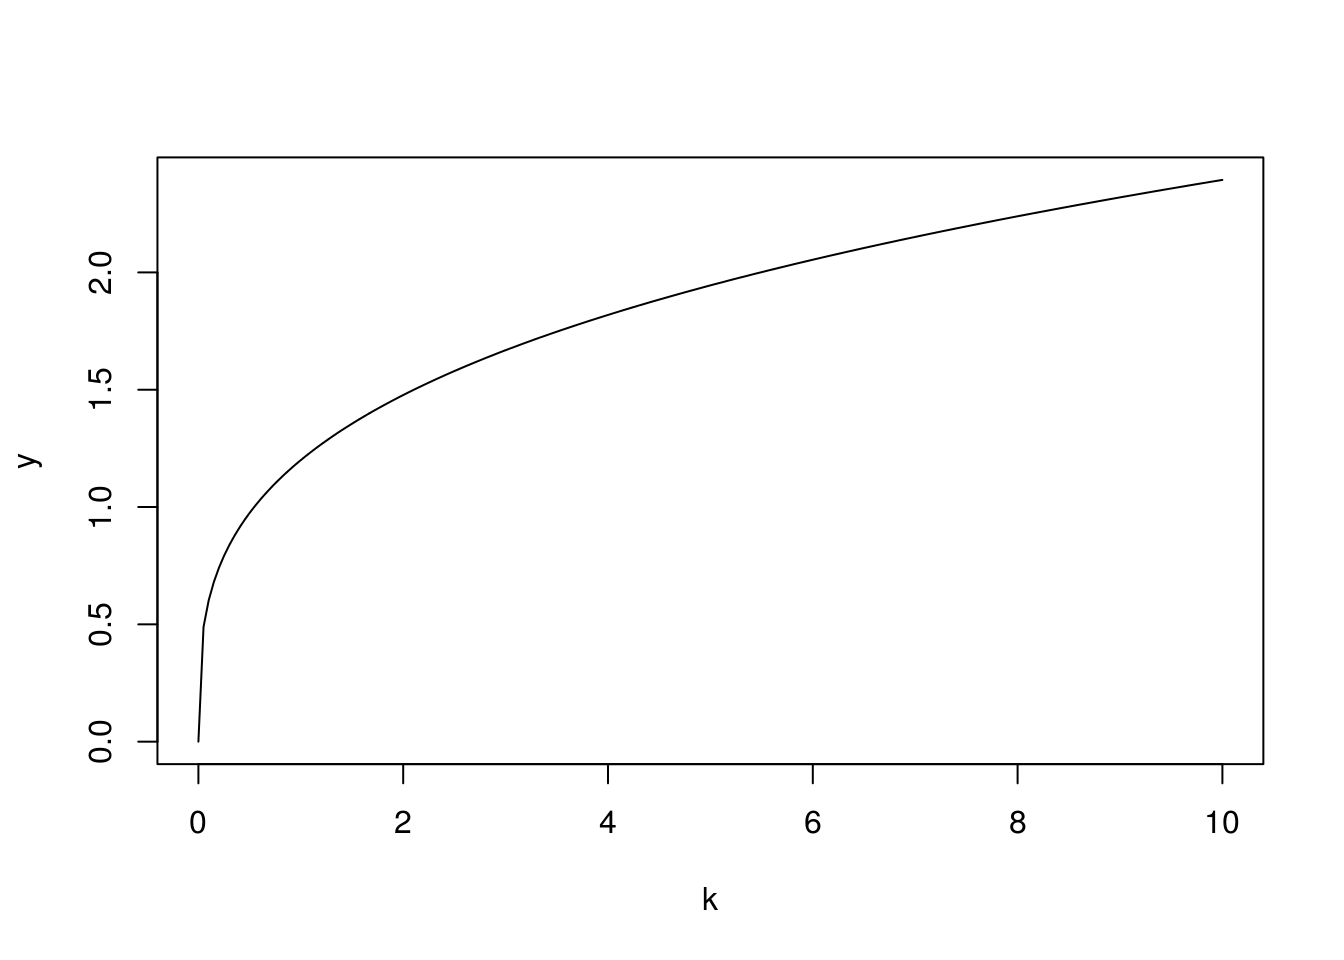
\includegraphics{linear-economic-dynamics_files/figure-latex/unnamed-chunk-5-1.pdf}
\caption{\label{fig:unnamed-chunk-5}`01\_cobbdouglas\_plot.R' の実行結果}
\end{figure}

\texttt{\#} に続く内容は, プログラマが読むためだけのコメントである.
本書の約束事として, コードチャンクの1行目のコメントには,
スクリプトとして保存する場合のファイル名や,
本文中で参照するための短いキャプションを書くことにする.

\subsubsection*{スクリプトファイル}
\addcontentsline{toc}{subsubsection}{スクリプトファイル}

スクリプトファイルを保存するディレクトリを作っておこう. Files
ペインを探して内容を見ると linear-economic-dynamics.Rproj
ファイルを見つけられる思う. そこがプロジェクトディレクトリの最上位階層
(ルートディレクトリ) である. もし当該ファイルが見当たらなければ,
ディレクトリ階層を移動して探してほしい.
元いた場所から離れることができたのだから戻ることもできるはずだ.
帰れなくなったら RStudio を終了して, 再び .Rproj
をダブルクリックして起動しなおせばよい.

プロジェクトの .Rpoj ファイルが見つかったら「New
Folder」というボタンを押して, 「R」という名前の新しいディレクトリを作る.

\textbf{スクリプト
(script)}とは1つ以上のコマンドをまとめたファイルのことである. R
はスクリプトファイルを読んで, 上から順番に実行することができる.
コンソール上での作業は複数行に渡るコードを入力するには不向きなので,
別途ファイルに保存しておくことで生

RStudio で新しいスクリプトファイルを作るにはいくつかの方法がある.

\begin{itemize}
\tightlist
\item
  RStudio 左上にあるるボタン (白い四角の上に足し算記号のマーク) から「R
  Script」を選びクリックする.
\item
  メニューから「File \textgreater{} New File \textgreater{} R
  Script」と進む.
\item
  \textbf{キーボードショートカット Ctrl+Shift+N / Cmd+Shift+N
  を押下する}
\end{itemize}

最後のキーボードショートカットを覚えるのが一番よいだろう. Cmd+Shit+N
を押下すると, Untitled1 という名前でソースペインが開く. ここに先程の
\texttt{01\_cobbdouglas\_plot.R} のコードをコピー&ペーストしてみよう.
Ctrl+S / Cmd+S によって保存しようとすると,
保存場所と名前を決めるように促されるので, 先程作成しておいた R
というフォルダに, \texttt{01\_cobbdouglas\_plot.R} という名前で配置する.
プロジェクトディレクトリは次のような構成になっているはずだ.\footnote{実際には
  .Rproj.user という隠しディレクトリがある.}

\begin{verbatim}
linear-economic-dynamics
├── R
│   └── 01_cobbdouglas_plot.R
└── linear-economic-dynamics.Rproj
\end{verbatim}

作業ディレクトリ (linear-economic-dynamics) にある, R
というサブディレクトリの中にある \texttt{01\_cobbdouglas\_plot.R}
というスクリプトファイルを実行するには以下のようにする.

\begin{Shaded}
\begin{Highlighting}[]
\KeywordTok{source}\NormalTok{(}\StringTok{'R/01_cobbdouglas_plot.R'}\NormalTok{)}
\end{Highlighting}
\end{Shaded}

作業ディレクトリを起点としたファイルの位置を\textbf{相対パス (relative
path)}という. スクリプト内にファイルパスを書く場合は,
やむを得ない事情で移動できない場合を除いて必ず相対パスで指定するようにする.

さきほどのスクリプトファイルはもっと下位のサブディレクトリに配置することもできる.
例えば, 章ごと節ごとにディレクトリを作って

\begin{verbatim}
source('R/part1/chapter03/section04/subsection01/01.R')
\end{verbatim}

ということも可能ではある. しかし,
階層が深くなりすぎると管理が難しくなるので,
できるだけフラットにしておくようにしよう. この本では,

\begin{verbatim}
R/chapternumber_descriptive_name.R
\end{verbatim}

という形式のファイル名をつけ, すべて R ディレクトリの直下に配置する.

\subsection{パッケージ}

\subsubsection*{tidyverse}\label{tidyverse}
\addcontentsline{toc}{subsubsection}{tidyverse}

本書では \texttt{tidyverse} パッケージを利用する. \texttt{tidyverse}
はRのデータフレーム操作を円滑にするためのパッケージ群である.
必要なもの以上に関数を読み込むことを望まない場合には, \texttt{ggplot2},
\texttt{dplyr}, \texttt{tidyr} を必要に応じて読み込むとよい.

試しにプロンプトに

\begin{Shaded}
\begin{Highlighting}[]
\KeywordTok{library}\NormalTok{(tidyverse)}
\end{Highlighting}
\end{Shaded}

と打ち込んでみよう.
エラーが出る場合には次のコマンドでインストールしてから, 再度実行する.

\begin{Shaded}
\begin{Highlighting}[]
\KeywordTok{install.packages}\NormalTok{(}\StringTok{"tidyverse"}\NormalTok{)}
\end{Highlighting}
\end{Shaded}

\begin{verbatim}
Loading tidyverse: ggplot2
Loading tidyverse: tibble
Loading tidyverse: tidyr
Loading tidyverse: readr
Loading tidyverse: purrr
Loading tidyverse: dplyr
Conflicts with tidy packages ---------------------------------------------------------
filter(): dplyr, stats
lag():    dplyr, stats
\end{verbatim}

といったメッセージが出ると思う. \texttt{tidyverse} はパッケージ群なので,
幾つかの個別のパッケージを読み込むのが仕事である. Conflicts
が出て心配になるかもしれないが, 特に問題はない. \texttt{filter()},
\texttt{lag()} という関数がデフォルトで読み込まれているにもかかわらず,
同じ名前を持つ \texttt{dplyr} を読み込んだことで\texttt{filter()},
\texttt{lag()} という関数の実体が変更されてしまった. もし,
\texttt{stats} を使いたければ, \texttt{stats::filter()}
と呼び出せばよい. \texttt{stats::} や \texttt{dplyr::}
といったプレフィックスは,
関数やオブジェクトがどのパッケージで定義されたものかを明示的にするときに使う.

本書では, \texttt{base::data.frame()} の代わりに
\texttt{tibble::tibble()} を利用する. \texttt{tibble} パッケージは
\texttt{tidyverse} に含まれている. 違いを簡単に見ておこう.

\begin{Shaded}
\begin{Highlighting}[]
\NormalTok{x =}\StringTok{ }\KeywordTok{c}\NormalTok{(}\DecValTok{1}\NormalTok{, }\DecValTok{2}\NormalTok{, }\DecValTok{3}\NormalTok{)}
\NormalTok{y =}\StringTok{ }\KeywordTok{c}\NormalTok{(}\StringTok{'a'}\NormalTok{, }\StringTok{'b'}\NormalTok{, }\StringTok{'c'}\NormalTok{)}
\NormalTok{z =}\StringTok{ }\KeywordTok{c}\NormalTok{(}\OtherTok{TRUE}\NormalTok{, }\OtherTok{TRUE}\NormalTok{, }\OtherTok{FALSE}\NormalTok{)}

\NormalTok{(}\DataTypeTok{df =} \KeywordTok{data.frame}\NormalTok{(}\DataTypeTok{x =} \NormalTok{x, }\DataTypeTok{y =} \NormalTok{y, }\DataTypeTok{z =} \NormalTok{z))}
\end{Highlighting}
\end{Shaded}

\begin{verbatim}
##   x y     z
## 1 1 a  TRUE
## 2 2 b  TRUE
## 3 3 c FALSE
\end{verbatim}

\begin{Shaded}
\begin{Highlighting}[]
\NormalTok{(}\DataTypeTok{tbl =} \KeywordTok{tibble}\NormalTok{(}\DataTypeTok{x =} \NormalTok{x, }\DataTypeTok{y =} \NormalTok{y, }\DataTypeTok{z =} \NormalTok{z))}
\end{Highlighting}
\end{Shaded}

\begin{verbatim}
## # A tibble: 3 × 3
##       x     y     z
##   <dbl> <chr> <lgl>
## 1     1     a  TRUE
## 2     2     b  TRUE
## 3     3     c FALSE
\end{verbatim}

base のデータフレームと比べて, tibble は次の点で扱いやすい.

\begin{itemize}
\tightlist
\item
  データのサイズを表示してくれる
\item
  コラムの型情報を表示する (\texttt{\textless{}dbl\textgreater{}},
  \texttt{\textless{}chr\textgreater{}},
  \texttt{\textless{}lgl\textgreater{}})
\item
  文字列をファクター型にしない
\end{itemize}

ファクター型は, 文字列を内部的に整数値として保存している.
これを文字列と思って扱うと問題が起こる. 例えば,

\begin{Shaded}
\begin{Highlighting}[]
\StringTok{"a"} \NormalTok{<}\StringTok{ "b"}
\end{Highlighting}
\end{Shaded}

\begin{verbatim}
## [1] TRUE
\end{verbatim}

と同じ振る舞いを期待して, 次のような評価をすると問題が起こる:

\begin{Shaded}
\begin{Highlighting}[]
\NormalTok{df$y[}\DecValTok{1}\NormalTok{] <}\StringTok{ }\NormalTok{df$y[}\DecValTok{2}\NormalTok{]}
\end{Highlighting}
\end{Shaded}

\begin{verbatim}
## Warning in Ops.factor(df$y[1], df$y[2]): '<' not meaningful for factors
\end{verbatim}

\begin{verbatim}
## [1] NA
\end{verbatim}

\subsubsection*{QZ}\label{qz}
\addcontentsline{toc}{subsubsection}{QZ}

同様に \texttt{QZ} パッケージもインストールしておこう.
後々利用することになる.

\begin{Shaded}
\begin{Highlighting}[]
\KeywordTok{install.packages}\NormalTok{(}\StringTok{"qz"}\NormalTok{)}
\end{Highlighting}
\end{Shaded}

\subsubsection*{devtools}\label{devtools}
\addcontentsline{toc}{subsubsection}{devtools}

パッケージ開発環境. \texttt{devtools::github\_install()} を使って,
github レポジトリからパッケージをインストールできるようになる.

\textbf{Step 1}:

コンパイラをインストールする.

\begin{itemize}
\tightlist
\item
  \textbf{Windows}:
  \href{https://cran.r-project.org/bin/windows/Rtools/}{Rtools
  (https://cran.r-project.org/bin/windows/Rtools/)} をインストール
\item
  \textbf{Mac}: Xcode をインストール
\end{itemize}

\textbf{Step 2}:

CRAN からインストール.

\begin{Shaded}
\begin{Highlighting}[]
\KeywordTok{install.packages}\NormalTok{(}\StringTok{"devtools"}\NormalTok{)}
\end{Highlighting}
\end{Shaded}

\chapter{複素数}\label{complexnumbers}

\section{はじめに}

マクロ経済学の導入的なトピックとして1セクターの最適成長理論を学び,
その後, 多セクターモデルを学ばないというケースもあるかもしれない.
1セクターモデルの典型的な成長経路は単調であり,
後の議論で明らかになるように,
このようなケースで複素数を考える必要はない. しかし,
応用上用いられるモデルの多くは複数のセクターと多数の内生変数によって構成される.
1セクターモデルのように単純な成長経路を描かない可能性がある. 例えば,
ある1点の周りを回転しながその点に接近するような経路を描くことがある.
このような現象を表現するには, 実数を考えるだけでは難しい.
経済モデルの動学を理解するには複素数の取扱いが必須なのである.\footnote{もちろんこれは経済変数が複素数値を取るということを意味しているのではない.
  実数パラメータのみで記述されるモデルに同等な変形を施して複素数値が現れる場合には,
  必ずその共役複素数が同時に現れ, 虚数部分を打ち消すように作用する.}

この節は,
経済学の学習の中で複素数に出会ったことのない人を対象とした入門的なトピックを扱っている.
上記のような話を具体的なモデルの中で説明できる読者は読み飛ばしても構わない.
あるいは, マクロ経済学が未修であっても,
行列の標準化の理論に明るい読者も読む必要がない.

\section{複素数}

実数 (real number) の集合を \(\mathbb R\) と書く. \(\mathbb R\)
に含まれない「数」を1つ追加し,
四則演算を自由にできるようにしたものが複素数 (complex number) の集合
\(\mathbb C\) になる.

追加する数は\textbf{虚数単位 (imaginary unit)}と呼ばれる. これは \[
  i^2 + 1 = 0
\] を成り立たせる \(i\) のことである. 実際にはそのような \(i\)
は複数ある (かもしれない) ので, そのうちの1つに \(i\)
という名前をつける. 実数の範囲にはこのような数は存在しないから, \(i\)
の追加によって \(\mathbb R\) より大きい集合を考えることになる.\footnote{2次関数
  \(x \mapsto x^2\) のグラフを考えてみればよい.}

\BeginKnitrBlock{definition}
\protect\hypertarget{def:unnamed-chunk-15}{}{\label{def:unnamed-chunk-15}}\textbf{複素数
(complex number)} とは, 実数 \(a\), \(b\) を用いて \[
  a + bi
\] と書ける数のことをいう. \(a\) を\textbf{実部 (real part)}, \(b\)
を\textbf{虚部 (imaginary part)} という.
\EndKnitrBlock{definition}

いつも \(a + bi\) のように書くと読みにくいので, \(z \in \mathbb C\)
に対して,

\begin{equation*}
   \mathrm{Re}~z = a, \qquad \mathrm{Im}~z = b
\end{equation*}

のような書き方をする.

複素数同士の四則演算を次のように定義する.

\BeginKnitrBlock{definition}
\protect\hypertarget{def:unnamed-chunk-16}{}{\label{def:unnamed-chunk-16}}
任意の \(a_1, a_2, b_1, b_2 \in \mathbb R\) に対して, \[
\begin{aligned}
  (a_1 + b_1 i) + (a_2 + b_2 i) &= (a_1 + a_2) + (b_1 + b_2) i \\
  (a_1 + b_1 i) - (a_2 + b_2 i) &= (a_1 - a_2) + (b_1 - b_2) i \\
  (a_1 + b_1 i) (a_2 + b_2 i) &= 
            (a_1 a_2 - b_1 b_2) + (a_1 b_2 + a_2 b_1 ) i.
\end{aligned}
\]

\(a_2 \neq 0\) または \(b_2 \neq 0\) であれば,

\[
\begin{aligned}
  \frac{a_1 + b_1 i}{a_2 + b_2 i}
    = 
    \left( \frac{a_1 a_2 + b_1 b_2}{a_2^2 + b_2^2} \right)
    +
    \left( \frac{- a_1 b_2 + a_2 b_1}{a_2^2 + b_2^2} \right) i.
\end{aligned}
\]
\EndKnitrBlock{definition}

\section{複素平面}

1つの複素数は \((a, b)\) という実数のペアと同一視できるので,
平面上の1点として複素数を表現できる.

\section{R コード}\label{r-}

R では複素数を簡単に使うことができる. 例えば次のように書くと, \texttt{z}
という名前の\textbf{変数}に \(5 + i\)
という複素数を代入するという意味になる. コンソールで実行してみてほしい.

\begin{Shaded}
\begin{Highlighting}[]
\NormalTok{z =}\StringTok{ }\DecValTok{5} \NormalTok{+}\StringTok{ }\NormalTok{1i}
\NormalTok{z}
\end{Highlighting}
\end{Shaded}

\begin{verbatim}
## [1] 5+1i
\end{verbatim}

\BeginKnitrBlock{exercise}
上のコードを次のように書き換えると正しく動くだろうか?何が起こるかを予想する.
その後, Rコンソールで実行して予想した結果と比べる.

\begin{itemize}
\tightlist
\item
  \texttt{1} と \texttt{i} の間にはスペースを入れる.
\item
  \texttt{1} を省略して \texttt{5\ +\ i} と書く.
\end{itemize}
\EndKnitrBlock{exercise}

\subsubsection*{実部}
\addcontentsline{toc}{subsubsection}{実部}

\texttt{Re()} によって実部を取得できる.

\begin{Shaded}
\begin{Highlighting}[]
\KeywordTok{Re}\NormalTok{(z)}
\end{Highlighting}
\end{Shaded}

\begin{verbatim}
## [1] 5
\end{verbatim}

\subsubsection*{虚部}
\addcontentsline{toc}{subsubsection}{虚部}

\texttt{Im()} によって虚部を取得できる.

\begin{Shaded}
\begin{Highlighting}[]
\KeywordTok{Im}\NormalTok{(z)}
\end{Highlighting}
\end{Shaded}

\begin{verbatim}
## [1] 1
\end{verbatim}

\subsection*{四則演算}
\addcontentsline{toc}{subsection}{四則演算}

四則演算も通常の数と同じようにできる.

\subsubsection*{加算}
\addcontentsline{toc}{subsubsection}{加算}

\begin{Shaded}
\begin{Highlighting}[]
\NormalTok{w =}\StringTok{ }\DecValTok{4} \NormalTok{-}\StringTok{ }\NormalTok{3i}
\NormalTok{z +}\StringTok{ }\NormalTok{w }
\end{Highlighting}
\end{Shaded}

\begin{verbatim}
## [1] 9-2i
\end{verbatim}

\subsubsection*{減算}
\addcontentsline{toc}{subsubsection}{減算}

\begin{Shaded}
\begin{Highlighting}[]
\NormalTok{z -}\StringTok{ }\NormalTok{w}
\end{Highlighting}
\end{Shaded}

\begin{verbatim}
## [1] 1+4i
\end{verbatim}

\subsubsection*{乗算}
\addcontentsline{toc}{subsubsection}{乗算}

\begin{Shaded}
\begin{Highlighting}[]
\NormalTok{z *}\StringTok{ }\NormalTok{w}
\end{Highlighting}
\end{Shaded}

\begin{verbatim}
## [1] 23-11i
\end{verbatim}

\subsubsection*{除算}
\addcontentsline{toc}{subsubsection}{除算}

\begin{Shaded}
\begin{Highlighting}[]
\NormalTok{z /}\StringTok{ }\NormalTok{w}
\end{Highlighting}
\end{Shaded}

\begin{verbatim}
## [1] 0.68+0.76i
\end{verbatim}

\subsubsection*{実数との演算}
\addcontentsline{toc}{subsubsection}{実数との演算}

実数と複素数の演算も自然に行うことができる.

\begin{Shaded}
\begin{Highlighting}[]
\DecValTok{10} \NormalTok{+}\StringTok{ }\NormalTok{z}
\end{Highlighting}
\end{Shaded}

\begin{verbatim}
## [1] 15+1i
\end{verbatim}

\subsection*{複素平面上の図示}
\addcontentsline{toc}{subsection}{複素平面上の図示}

\subsubsection*{ggplot2 による作図の基本}\label{ggplot2-}
\addcontentsline{toc}{subsubsection}{ggplot2 による作図の基本}

base R の \texttt{plot()} 関数は複素数に対応しているが, 残念ながら
\texttt{ggplot2} はそのようにはできていない. とは言っても
\texttt{ggplot2} を使うことを推奨する.

まず実部と虚部を分けてデータフレームに保存しておく. base R の
\texttt{data.frame()} ではなく \texttt{tidyverse} パッケージ
(\texttt{tibble} パッケージ) の \texttt{tibble()} を用いる. tibble
データフレームもデータフレームと呼ぶ.

\begin{Shaded}
\begin{Highlighting}[]
\NormalTok{points =}\StringTok{ }
\StringTok{  }\KeywordTok{tibble}\NormalTok{(}\DataTypeTok{z =} \KeywordTok{c}\NormalTok{(z, w, z /}\StringTok{ }\NormalTok{w)) %>%}\StringTok{ }
\StringTok{  }\KeywordTok{mutate}\NormalTok{(}\DataTypeTok{re =} \KeywordTok{Re}\NormalTok{(z), }\DataTypeTok{im =} \KeywordTok{Im}\NormalTok{(z))}
\NormalTok{points}
\end{Highlighting}
\end{Shaded}

\begin{verbatim}
## # A tibble: 3 × 3
##            z    re    im
##       <cplx> <dbl> <dbl>
## 1 5.00+1.00i  5.00  1.00
## 2 4.00-3.00i  4.00 -3.00
## 3 0.68+0.76i  0.68  0.76
\end{verbatim}

今作ったデータフレームの \texttt{re} 列を横軸に, \texttt{im}
列を縦軸にプロットすればよい.

\begin{Shaded}
\begin{Highlighting}[]
\KeywordTok{ggplot}\NormalTok{(points) +}\StringTok{ }\KeywordTok{geom_point}\NormalTok{(}\KeywordTok{aes}\NormalTok{(}\DataTypeTok{x=}\NormalTok{re, }\DataTypeTok{y=}\NormalTok{im, }\DataTypeTok{color=}\KeywordTok{factor}\NormalTok{(z))) +}\StringTok{ }
\StringTok{  }\KeywordTok{coord_fixed}\NormalTok{() +}\StringTok{ }\KeywordTok{xlim}\NormalTok{(-}\DecValTok{5}\NormalTok{, }\DecValTok{5}\NormalTok{) +}\StringTok{ }\KeywordTok{ylim}\NormalTok{(-}\DecValTok{5}\NormalTok{, }\DecValTok{5}\NormalTok{) }\CommentTok{# この行は装飾}
\end{Highlighting}
\end{Shaded}

\includegraphics{linear-economic-dynamics_files/figure-latex/unnamed-chunk-27-1.pdf}

\subsubsection*{べき乗}
\addcontentsline{toc}{subsubsection}{べき乗}

上の方法をもう少し工夫してみよう. 同じ複素数を繰り返し掛けてみよう. \[
  z_p = 0.5 + 0.5i
\] として, \(z_p^n\) を計算しよう. ただし, \(z_p^n\) は \(z_p\)
のべき乗で, 実数と同様 \(z_p^0 = 1\), \(z_p^n = z_p z_p^{n-1}\),
\(n > 1\) と定義する.

\begin{Shaded}
\begin{Highlighting}[]
\NormalTok{zp =}\StringTok{ }\FloatTok{0.5} \NormalTok{+}\StringTok{ }\FloatTok{0.}\NormalTok{5i}
\NormalTok{zn =}\StringTok{ }\KeywordTok{tibble}\NormalTok{(}\DataTypeTok{re =} \KeywordTok{Re}\NormalTok{(}\DecValTok{1}\NormalTok{), }\DataTypeTok{im =} \KeywordTok{Im}\NormalTok{(}\DecValTok{1}\NormalTok{), }\DataTypeTok{n =} \DecValTok{0}\NormalTok{)}

\NormalTok{for (i in }\DecValTok{1}\NormalTok{:}\DecValTok{10}\NormalTok{) \{}
  \NormalTok{zn =}\StringTok{ }\NormalTok{zn %>%}\StringTok{ }\KeywordTok{add_row}\NormalTok{(}\DataTypeTok{re =} \KeywordTok{Re}\NormalTok{(zp ^}\StringTok{ }\NormalTok{i), }\DataTypeTok{im =} \KeywordTok{Im}\NormalTok{(zp ^}\StringTok{ }\NormalTok{i), }\DataTypeTok{n =} \NormalTok{i)}
\NormalTok{\}}

\KeywordTok{ggplot}\NormalTok{(zn) +}\StringTok{ }\KeywordTok{geom_point}\NormalTok{(}\KeywordTok{aes}\NormalTok{(}\DataTypeTok{x=}\NormalTok{re, }\DataTypeTok{y=}\NormalTok{im, }\DataTypeTok{color=}\KeywordTok{factor}\NormalTok{(n))) +}\StringTok{ }
\StringTok{  }\KeywordTok{coord_fixed}\NormalTok{() +}\StringTok{ }\KeywordTok{xlim}\NormalTok{(-}\FloatTok{1.02}\NormalTok{, }\FloatTok{1.02}\NormalTok{) +}\StringTok{ }\KeywordTok{ylim}\NormalTok{(-}\FloatTok{1.02}\NormalTok{, }\FloatTok{1.02}\NormalTok{)}
\end{Highlighting}
\end{Shaded}

\includegraphics{linear-economic-dynamics_files/figure-latex/unnamed-chunk-28-1.pdf}

\(1\) に \(0.5 + 0.5i\)
を繰り返し掛けると次第に原点に近づいていくことが分かる. これは,
実部・虚部ともに \(0.5\)
という比較的小さな数字だから成り立ちそうな気がする. 実数の場合,
\(\lim_{n\to \infty} a^n = 0\) となるのは, \(-1 < a < 1\)
の場合ということを思いだしてほしい. 複素数の場合には,
実部・虚部のそれぞれが\(1\)
より小さい絶対値を持てば原点に収束するだろうか?

例えば次の例を考えてみよう. \[
  z_q = 0.9 + 0.9i
\] はたして \(z_q^n\) は原点に収束するだろうか?

\begin{Shaded}
\begin{Highlighting}[]
\NormalTok{zq =}\StringTok{ }\FloatTok{0.9} \NormalTok{+}\StringTok{ }\FloatTok{0.}\NormalTok{9i}
\NormalTok{zm =}\StringTok{ }\KeywordTok{tibble}\NormalTok{(}\DataTypeTok{re =} \KeywordTok{Re}\NormalTok{(}\DecValTok{1}\NormalTok{), }\DataTypeTok{im =} \KeywordTok{Im}\NormalTok{(}\DecValTok{1}\NormalTok{), }\DataTypeTok{n =} \DecValTok{0}\NormalTok{)}

\NormalTok{for (i in }\DecValTok{1}\NormalTok{:}\DecValTok{10}\NormalTok{) \{}
  \NormalTok{zm =}\StringTok{ }\NormalTok{zm %>%}\StringTok{ }\KeywordTok{add_row}\NormalTok{(}\DataTypeTok{re =} \KeywordTok{Re}\NormalTok{(zq ^}\StringTok{ }\NormalTok{i), }\DataTypeTok{im =} \KeywordTok{Im}\NormalTok{(zq ^}\StringTok{ }\NormalTok{i), }\DataTypeTok{n =} \NormalTok{i)}
\NormalTok{\}}

\KeywordTok{ggplot}\NormalTok{(zm) +}\StringTok{ }\KeywordTok{geom_point}\NormalTok{(}\KeywordTok{aes}\NormalTok{(}\DataTypeTok{x=}\NormalTok{re, }\DataTypeTok{y=}\NormalTok{im, }\DataTypeTok{color=}\KeywordTok{factor}\NormalTok{(n))) +}\StringTok{ }
\StringTok{  }\KeywordTok{coord_fixed}\NormalTok{() +}\StringTok{ }\KeywordTok{xlim}\NormalTok{(-}\DecValTok{12}\NormalTok{, }\DecValTok{12}\NormalTok{) +}\StringTok{ }\KeywordTok{ylim}\NormalTok{(-}\DecValTok{12}\NormalTok{, }\DecValTok{12}\NormalTok{)}
\end{Highlighting}
\end{Shaded}

\includegraphics{linear-economic-dynamics_files/figure-latex/unnamed-chunk-29-1.pdf}

上の図を見る限り, 回転しながらどんどん原点から離れていっているようだ.
原点への収束, 原点からの乖離はどのような条件で特徴付けられるだろうか.

\section{極形式}

複素数のべき乗を計算するということは \(1\)
に同じ複素数を繰り返し掛けることに外ならない. その結果として,
上で描いた2つの図のように回転と拡大・縮小という現象を確認することができた.

複素数 \(z = a + bi\) を平面上の点 \((a, b)\) とみなせるというのが,
複素平面を描いた際に念頭に置いていた事実であった. さらに平面上の点
\((a, b)\) は原点からの距離と 矢線ベクトル \((1, 0)\)
を基準とした回転角で表せるということを思い出してほしい. つまり, ある
\(0 \le \theta < 360^\circ\) が存在して次の等式が成立する. \[
\begin{aligned}
  a = \sqrt{a^2 + b^2} \cos \theta\\
  b = \sqrt{a^2 + b^2} \sin \theta\\
\end{aligned}
\]

\(r = \sqrt{a^2 + b^2}\ge 0\) を \(z = a + bi\) の\textbf{絶対値
(absolute value)}という. \(z\) の絶対値を \(|z|\) で表す. \(\theta\)
を\textbf{偏角 (argument)} という (\(\mathrm{arg}(z)\)
で表すこともある). すべての複素数が \[
  z = r(\cos\theta + i\sin\theta)
\] という表現を持つ. この表現を複素数の\textbf{極形式 (polar
form)}という.

絶対値が\(1\) で偏角の異なる2つの複素数 \(\cos\theta_1 + i\sin\theta_1\)
と \(\cos\theta_2 + i\sin\theta_2\) を掛け合わせると

\begin{align}
  &(\cos\theta_1 + i\sin\theta_1)(\cos\theta_2 + i\sin\theta_2) \notag \\
  &\qquad=
  (\cos\theta_1 \cos\theta_2 - \sin\theta_1\sin\theta_2)
  +
  i(\sin\theta_1\cos\theta_2 + \cos\theta_1\sin\theta_2) \notag \\
  &\qquad=
  \cos(\theta_1 + \theta_2) + i\sin(\theta_1 + \theta_2) \label{eq:polar}
\end{align}

を得る.\footnote{加法定理を使った.} 絶対値が\(1\)でない場合にも,
\(r_1, r_2 > 0\) として, \[
\begin{aligned}
  r_1(\cos\theta_1 + i\sin\theta_1)\cdot r_2(\cos\theta_2 + i\sin\theta_2)
  =
  r_1 r_2 \left[
    \cos(\theta_1 + \theta_2) + i\sin(\theta_1 + \theta_2)
  \right]
\end{aligned}
\] つまり, 複素数 \(r_2(\cos\theta_2 + i\sin\theta_2)\)
を掛けるという操作は, 絶対値を \(r_2\) 倍に伸縮し, 偏角を \(+\theta_2\)
だけ回転させる作用がある.

\subsubsection*{オイラーの公式}
\addcontentsline{toc}{subsubsection}{オイラーの公式}

式\eqref{eq:polar} は複素数の積が偏角の和に相当することを述べている.
この等式を眺めて指数関数との関連性に気がつく人もいるかもしれない. 実際,

\begin{align}
  e^{i\theta} = \cos\theta + i\sin\theta \label{eq:euler}
\end{align}

と定義すれば, 指数法則 \[
  e^{i\theta_1} e^{i\theta_2} = e^{i(\theta_1 + \theta_2)}
\]

によって, 式\eqref{eq:polar} を「導出」できる. 本来は, \(e^{i\theta}\)
が意味するところをきちんと定義して, 等式 \eqref{eq:euler}
を証明する必要があるだろうが,
ここでは記号として「オイラーの公式」を紹介した.
関心のある読者は適当な複素関数論の教科書を読めばよい.

すべての複素数が

\begin{equation}
  z = re^{i\theta}, \quad r \ge 0,\ 0^\circ \le \theta < 360^\circ
\end{equation}

という表現を持つということを知っていればよい. なお,
この表現は次のようにして, \(\theta < 0^\circ\), \(\theta \ge 360^\circ\)
に拡張することができる: 任意の \(\theta\) に対して,
\(\theta = \theta_0 + n \times 360^\circ\) なる整数
\(n = 0, \pm 1, \pm 2, \dots\) がたった1つだけ存在する.
\(e^{i360^\circ} = 1\) に注意すれば,

\begin{equation}
  e^{i\theta} = e^{i\theta_0}\left(e^{i360^\circ}\right)^n = e^{i\theta_0}
\end{equation}

を得る.

\subsubsection*{べき乗}\label{-1}
\addcontentsline{toc}{subsubsection}{べき乗}

以上の準備の下で, \[
\begin{aligned}
  \lim_{n\to\infty} z_p^n  = (0.5 + 0.5i)^n \to 0,
  \quad \text{and}\quad
  \lim_{n\to\infty} z_q^n = (0.9 + 0.9i)^n \not\to 0
\end{aligned}
\] について説明することができる.

極形式による表現 \[
\begin{aligned}
  z_p = r_p e^{i\theta_p}\\
  z_q = r_q e^{i\theta_q}
\end{aligned}
\] によれば, \[
\begin{aligned}
  r_p = \sqrt{0.5^2 + 0.5^2} \simeq 0.7071068 < 1\\ 
  r_q = \sqrt{0.9^2 + 0.9^2} \simeq 1.2727922 > 1.
\end{aligned}
\] したがって, \[
\begin{aligned}
  |z_p^n| &= |r_p^n e^{i n\theta_p}| = r_p^n \to 0\\
  |z_q^n| &= |r_q^n e^{i n\theta_q}| = r_q^n \to \infty
\end{aligned}
\] を得る. この観察をまとめておこう.

\BeginKnitrBlock{fact}
\begin{itemize}
\tightlist
\item
  \(|z| < 1\) ならば \(\lim_{n\to\infty} |z^n| = 0\),
\item
  \(|z| > 1\) ならば \(\lim_{n\to\infty} |z^n| = \infty\),
\item
  \(|z| = 1\) ならば 任意の \(n\) について \(|z^n| = 1\).
\end{itemize}
\EndKnitrBlock{fact}

\section{共役複素数}

複素数 \(z = a + bi\) に対して, \(\bar z = a - bi\) を\textbf{共役複素数
(complex conjugate)}あるいは\textbf{複素共役}という. \(z\) は \(\bar z\)
の共役複素数であるから,

\begin{equation*}
  \bar{\bar z} = z 
\end{equation*}

が成り立つ. また, \BeginKnitrBlock{exercise}

任意の複素数 \(z\) に対して, \[
  z\bar z = |z|^2
\] を示せ.
\EndKnitrBlock{exercise}

R では, \texttt{Conj()} で複素共役を, \texttt{abs()}
で複素数の絶対値を計算できる.

\begin{Shaded}
\begin{Highlighting}[]
\NormalTok{z}
\end{Highlighting}
\end{Shaded}

\begin{verbatim}
## [1] 5+1i
\end{verbatim}

\begin{Shaded}
\begin{Highlighting}[]
\KeywordTok{Conj}\NormalTok{(z)}
\end{Highlighting}
\end{Shaded}

\begin{verbatim}
## [1] 5-1i
\end{verbatim}

\begin{Shaded}
\begin{Highlighting}[]
\KeywordTok{abs}\NormalTok{(z)}
\end{Highlighting}
\end{Shaded}

\begin{verbatim}
## [1] 5.09902
\end{verbatim}

先程の練習問題の性質は \texttt{z\ *\ Conj(z)} と
\texttt{abs(z)\ \^{}\ 2} の差が十分ゼロに近いことで確認できる.

\begin{Shaded}
\begin{Highlighting}[]
\NormalTok{z *}\StringTok{ }\KeywordTok{Conj}\NormalTok{(z) -}\StringTok{ }\KeywordTok{abs}\NormalTok{(z) ^}\StringTok{ }\DecValTok{2}
\end{Highlighting}
\end{Shaded}

\begin{verbatim}
## [1] 3.552714e-15+0i
\end{verbatim}

\texttt{e-15} というのは, \texttt{10\^{}\{-15\}} を意味しているので,
大変小さい数字であることが分かるだろう. あるいは, 次の様にすればよい.

\begin{Shaded}
\begin{Highlighting}[]
\KeywordTok{all.equal}\NormalTok{(z *}\StringTok{ }\KeywordTok{Conj}\NormalTok{(z), }\KeywordTok{abs}\NormalTok{(z)^}\StringTok{ }\DecValTok{2} \NormalTok{+}\StringTok{ }\NormalTok{0i)}
\end{Highlighting}
\end{Shaded}

\begin{verbatim}
## [1] TRUE
\end{verbatim}

計算機上の小数 (浮動小数点数)
は実数を有限近似したものに過ぎないので等号で評価することはできない.
有限の長さを持つように見えるありきたりな有理数でさえ,
等号による評価はあてにならない. 例えば次のような例がある. 

\begin{Shaded}
\begin{Highlighting}[]
\NormalTok{sum =}\StringTok{ }\DecValTok{0}
\NormalTok{for (i in }\DecValTok{1}\NormalTok{:}\DecValTok{10}\NormalTok{) \{}
  \NormalTok{sum =}\StringTok{ }\NormalTok{sum +}\StringTok{ }\FloatTok{0.1}
\NormalTok{\}}
\NormalTok{sum ==}\StringTok{ }\DecValTok{1}
\end{Highlighting}
\end{Shaded}

\begin{verbatim}
## [1] FALSE
\end{verbatim}

0.1 を 10回足しても 1 にはならない. 小数の比較に \texttt{==}
を用いてはいけない.

\subsubsection*{多項式方程式の解}
\addcontentsline{toc}{subsubsection}{多項式方程式の解}

後ほど明らかになるように,
線形システムは固有多項式と呼ばれる実係数多項式を「因数分解」する問題を通じて分析される.
あるいは, 本質的には同じことだが, 実係数多項式方程式の解を調べる.
いずれにせよ実係数多項式方程式が重要な役割を果たす.

多項式方程式は次のような性質を持つ. \BeginKnitrBlock{theorem}

\protect\hypertarget{thm:unnamed-chunk-36}{}{\label{thm:unnamed-chunk-36}}\(a_n, \dots, a_0 \in \mathbb R\)
とする. \(z\) の多項式 \[
  p(z) = a_n z^n + a_{n-1} z^{n-1} + \cdots + a_1 z + a_0
\] が\(z_0 \in \mathbb C\) で \(p(z_0) = 0\) を満たせば,
\(p(\bar z_0) = 0\) が成り立つ.
\EndKnitrBlock{theorem}

適当な代数学・複素関数論の本を参照のこと. この性質をもって \(\mathbb C\)
は\textbf{代数的閉体}であると言われる.\footnote{その集合の元を係数とする多項式方程式の解がその集合に含まれる.
  実係数方程式 \(x^2 + 1 = 0\) は実数の解を持たないので,
  実数は代数的閉体ではない.} さらに係数を実数に制限すれば,
次の定理を証明できる.

\BeginKnitrBlock{theorem}
\protect\hypertarget{thm:unnamed-chunk-37}{}{\label{thm:unnamed-chunk-37}}\(a_n, \dots, a_0 \in \mathbb R\)
とする. \(z\) の多項式 \[
  p(z) = a_n z^n + a_{n-1} z^{n-1} + \cdots + a_1 z + a_0
\] が\(z_0 \in \mathbb C\) で \(p(z_0) = 0\) を満たせば,
\(p(\bar z_0) = 0\) が成り立つ.
\EndKnitrBlock{theorem}

\BeginKnitrBlock{proof}
\iffalse {証明. } \fi 任意の \(a \in \mathbb R\) に対して\(\bar a = a\)
であることと, \(\overline{z^n} = (\bar z)^n\) に注意する.
\(\overline{p(z)} = p(\bar z)\) が成り立つので, \(p(z) = 0\) ならば
\(p(\bar z) = 0\) が言える.
\EndKnitrBlock{proof}

\chapter{線形代数}\label{matrix}

学部初年次の線形代数学で学ぶ重要項目について幾つかピックアップしたものである.
経済動学の学習に必要な項目を取り上げているが,
十分に網羅的になっている訳ではないので,
線形代数学の成書を1つ手元に置いておくのがよいと思う.

\section{行列の形}

システムの振る舞いをよりよく理解するためには抽象的な線形空間論まで踏み込む必要があるが,
それは次回以降に譲って, ここでは表形式に数を並べたものとして\textbf{行列
(matrix)} を捉えよう. 従って, 行列とは次のような対象である. \[
A=\begin{bmatrix}a_{1,1} & a_{1,2} & \cdots & a_{1,n-1} & a_{1,n}\\
a_{2,1} & a_{2,2} & \cdots & a_{2,n-1} & a_{2,n}\\
\vdots & \vdots & \ddots & \vdots & \vdots\\
a_{m-1,1} & a_{m-1,2} & \cdots & a_{m-1,n-1} & a_{m-1,n}\\
a_{m,1} & a_{m,2} & \cdots & a_{m-1,n} & a_{m,n}
\end{bmatrix}
\]

ただし, \(a_{i,j}\in\mathbb{F}\), \(i=1,\dots,m\), \(j=1,\dots,n\).
\(\mathbb{F}\) は \(\mathbb{R}\) または \(\mathbb{C}\). 数 \(a_{i,j}\)
を行列の\textbf{成分}または\textbf{要素 (element, component, entry)}
と呼ぶ. 混乱の恐れがない場合はコンマを外して \(a_{ij}\)
と書くことが多い. 成分を明らかにするための簡略表記として \(A=[a_{ij}]\)
といった書き方をする場合がある. また, 行列 \(A\) の \((i,j)\) 成分
\(a_{ij}\) を\(A_{ij}\) のように書くこともある.

各\\
\[
\begin{aligned}
  &\begin{bmatrix}a_{1,1} & a_{1,2} & \cdots & a_{1,n-1} & a_{1,n}\end{bmatrix}\\
  &\begin{bmatrix}a_{2,1} & a_{2,2} & \cdots & a_{2,n-1} & a_{2,n}\end{bmatrix}\\
  &\hspace{6em}\vdots\\
  &\begin{bmatrix}a_{m,1} & a_{m,2} & \cdots & a_{m,n-1} & a_{m,n}\end{bmatrix}
\end{aligned}
\]\\
を行列の\textbf{行 (row)} という. 一方, 各 \[
\begin{bmatrix}a_{1,1}\\
a_{2,1}\\
\vdots\\
a_{m-1,1}\\
a_{m,1}
\end{bmatrix},\ \begin{bmatrix}a_{1,2}\\
a_{2,2}\\
\vdots\\
a_{m-1,2}\\
a_{m,2}
\end{bmatrix},\ \dots,\ \begin{bmatrix}a_{1,n}\\
a_{2,n}\\
\vdots\\
a_{m-1,n}\\
a_{m,n}
\end{bmatrix}
\]

を行列の\textbf{列 (column)} という. 上の行列\(A\)
は\(m\)個の行と\(n\)個の列を持つので, \(m\times n\) 行列と呼ばれる.
\(\mathbb{F}^{m\times n}\) を \(\mathbb{F}\) の値を成分にもつ
\(m\times n\) 行列の全体の集合と定義する.

行列の形にまつわるいくつかの用語を確認しておこう.

\subsubsection*{正方行列 (square matrix)}\label{-square-matrix}
\addcontentsline{toc}{subsubsection}{正方行列 (square matrix)}

\(m=n\) のとき, すなわち \(A\in\mathbb{F}^{n\times n}\) のとき, \(A\) は
\(n\) 次の\textbf{正方行列 (square matrix of order \(n\))} であるいう.

\subsubsection*{ゼロ行列 (zero matrix, null
matrix)}\label{-zero-matrix-null-matrix}
\addcontentsline{toc}{subsubsection}{ゼロ行列 (zero matrix, null
matrix)}

すべての成分がゼロである行列をゼロ行列という. サイズが \(m\times n\)
であるゼロ行列を \(0_{m\times n}\) とか \(O_{m\times n}\) と書く.
多くの場合にそうであるように, 混乱の恐れがない場合には \(O\) とか \(0\)
と書く.

\subsubsection*{対角成分 (diagonal elements)}\label{-diagonal-elements}
\addcontentsline{toc}{subsubsection}{対角成分 (diagonal elements)}

正方行列 \(A\) の成分 \(\{a_{ij}\ |\ i,j=1,\dots,n\}\) のうち \(i=j\)
なる部分 \(\{a_{11},\dots,a_{nn}\}\) を\textbf{対角成分 (diagonal
element)}という. 対角成分の1つ上の成分
\(\{a_{12},a_{23},\dots,a_{n-1,n}\}\) を\textbf{優対角成分
(superdiagonal element)}, 対角成分の1つ下の成分
\(\{a_{21},a_{32},\dots,a_{n,n-1}\}\) を\textbf{劣対角成分 (subdiagonal
element)} という. 対角成分の和を\textbf{トレース (trace)} といい,
\(\mathrm{trace}A\) と書く.

\subsubsection*{三角行列 (triangular matrix)}\label{-triangular-matrix}
\addcontentsline{toc}{subsubsection}{三角行列 (triangular matrix)}

正方行列\(A=[a_{ij}]\) が \(i>j\Rightarrow a_{ij}=0\) を満たすとき,
\(A\) を\textbf{上三角行列 (upper triangular matrix)} という. 一方,
\(A=[a_{ij}]\) が \(i<j\Rightarrow a_{ij}=0\) を満たすとき, \(A\)
は\textbf{下三角行列 (lower triangular matrix)} であるという.
上三角行列は対角成分より下にある成分がすべてゼロ,
下三角行列は対角成分より上にある成分がすべてゼロである.

\subsubsection*{対角行列 (diagonal matrix)}\label{-diagonal-matrix}
\addcontentsline{toc}{subsubsection}{対角行列 (diagonal matrix)}

対角成分を除いた成分がすべてゼロであるような正方行列を\textbf{対角行列
(diagonal matrix)}という. ときに, \(\mathrm{diag}\{a_{1},\dots,a_{n}\}\)
のように書いて対角成分が左上から順に \(a_{1},\dots,a_{n}\)
である対角行列を表すことがある. これは Matlab
などで利用されている記法で, Python と Octave でも利用できる.

\subsubsection*{単位行列 (identity matrix)}\label{-identity-matrix}
\addcontentsline{toc}{subsubsection}{単位行列 (identity matrix)}

対角成分がすべて\(1\) である対角行列を単位行列という.
\(n\)次の単位行列を \(I_{n}\) と書く. 誤解の恐れがない場合は単に \(I\)
と書く. Python では関数 numpy.eye(n) で \(n\) 次単位行列を作る.

\subsubsection*{転置行列 (transpose matrix)}\label{-transpose-matrix}
\addcontentsline{toc}{subsubsection}{転置行列 (transpose matrix)}

\(A=[a_{ij}]\in\mathbb{F}^{m\times n}\) の転置行列 \(A^{\top}\) とは,
\((A^{\top})_{ij}=a_{ji}\), \(i=1,\dots,m\), \(j=1,\dots n\)
を満たす\(m\times n\)行列のことをいう.

\subsubsection*{共役転置行列 (conjugate
transpose)}\label{-conjugate-transpose}
\addcontentsline{toc}{subsubsection}{共役転置行列 (conjugate transpose)}

\(A=[a_{ij}]\in\mathbb{F}^{m\times n}\) の共役転置行列 \(A^{*}\) とは,
\((A^{*})_{ij}=\bar{a}_{ji}\), \(i=1,\dots,m\), \(j=1,\dots n\)
を満たす\(m\times n\)行列のことである.
実行列の共役転置行列は転置行列である.

\subsubsection*{対称行列 (symmetric matrix)}\label{-symmetric-matrix}
\addcontentsline{toc}{subsubsection}{対称行列 (symmetric matrix)}

\(A\in\mathbb{R}^{n\times n}\) が\textbf{対称行列 (symmetric
matrix)}であるとは, \(A^{\top}=A\) が成り立つことをいう.

\subsubsection*{エルミート行列 (Hermitian
matrix)}\label{-hermitian-matrix}
\addcontentsline{toc}{subsubsection}{エルミート行列 (Hermitian matrix)}

\(A\in\mathbb{C}^{n\times n}\) がエルミート行列であるとは, \(A^{*}=A\)
が成り立つことをいう.

\subsubsection*{列ベクトル・行ベクトル (column vector, row
vector)}\label{-column-vector-row-vector}
\addcontentsline{toc}{subsubsection}{列ベクトル・行ベクトル (column
vector, row vector)}

のちに見るように行列の集合には元どうしの加法とスカラー倍が定義され,
それらは望ましい性質を満たす.
ゼロ元・逆元と呼ばれる特別な元の存在も自明であるので,
特定のサイズの行列全体の集合は, (のちに定義する)
ベクトル空間の一例となっている. 特に \[
  \mathbb{F}^{n\times1},\quad\mathbb{F}^{1\times n}
\] は我々が頻繁に用いる有限次元ベクトル空間の表現となっている.
通常これらのうちいずれかを \(\mathbb{F}^{n}\) と記す. 一般の
\(A\in\mathbb{F}^{n\times m}\) を\(n\)次元列ベクトル
(\(\mathbb{F}^{n\times1})\) を \(m\) 個並べたものと捉えたり,
\(m\)次元列ベクトル (\(\mathbb{F}^{1\times m})\) を \(n\)
個並べたものと捉えたりすることがある.

\subsubsection*{ブロック行列 (block matrix)}\label{-block-matrix}
\addcontentsline{toc}{subsubsection}{ブロック行列 (block matrix)}

行列をいくつかの部分行列に分解した上で分析する方が都合の良い場合がある.
例えば, \[
A=\left[
  \begin{array}{ccc|ccc}
    a_{1,1} & \cdots & a_{1,n} & a_{1,n+1} & \cdots & a_{1,n+q}\\
    \vdots & \ddots & \vdots & \vdots & \ddots & \vdots\\
    a_{m,1} & \cdots & a_{m,n} & a_{m,n+1} & \cdots & a_{m,n+q}\\
    \hline a_{m+1,1} & \cdots & a_{m+1,n} & a_{m+1,n+1} & \cdots & a_{m+1,n+q}\\
    \vdots & \ddots & \vdots & \vdots & \ddots & \vdots\\
    a_{m+p,1} & \cdots & a_{m+p,n} & a_{m+p,n+1} & \cdots & a_{m+p,n+q}
  \end{array}
  \right]
  =:
  \left[
    \begin{array}{c|c}
      A_{11} & A_{12}\\
      \hline 
      A_{21} & A_{22}
    \end{array}
  \right]
\] のように, 大きな行列 \(A\in\mathbb{F}^{(m+p)\times(n+q)}\)
を4つの部分行列 \(A_{11}\in\mathbb{F}^{m\times n}\),
\(A_{12}\in\mathbb{F}^{m\times q}\),
\(A_{21}\in\mathbb{F}^{p\times n}\), \(A_{22}\in\mathbb{F}^{p\times q}\)
に分解するなどである.\footnote{\(P:=Q\) という表現は, \(P\) を \(Q\)
  で定義するという意味, \(P =:Q\) は \(Q\) を\(P\)
  で定義するという意味である.} \(A_{12}=0\), \(A_{21}=0\) であるとき,
\textbf{ブロック対角行列 (block diagonal matrix)}であるといい,
\(A_{21}=0\) であるとき\textbf{ブロック上三角行列 (block upper
triangular matrix)}であるなどという.

\section{行列の演算}

\subsubsection*{スカラー倍}
\addcontentsline{toc}{subsubsection}{スカラー倍}

\(A\in\mathbb{F}^{m\times n}\) に対してスカラー倍 (scalar
multiplication) あるいは定数倍と呼ばれる操作が次のように定義される:
\(\alpha\in\mathbb{F}\) について, \[
\alpha A:=\begin{bmatrix}\alpha a_{1,1} & \alpha a_{1,2} & \cdots & \alpha a_{1,n-1} & \alpha a_{1,n}\\
\alpha a_{2,1} & \alpha a_{2,2} & \cdots & \alpha a_{2,n-1} & \alpha a_{2,n}\\
\vdots & \vdots & \ddots & \vdots & \vdots\\
\alpha a_{m-1,1} & \alpha a_{m-1,2} & \cdots & \alpha a_{m-1,n-1} & \alpha a_{m-1,n}\\
\alpha a_{m,1} & \alpha a_{m,2} & \cdots & \alpha a_{m-1,n} & \alpha a_{m,n}
\end{bmatrix}\in\mathbb{F}^{m\times n}.
\]

\subsubsection*{和}
\addcontentsline{toc}{subsubsection}{和}

同数の行と列を持つ2つの行列に対して次のようにして和が定義できる.
\(A=[a_{ij}]\in\mathbb{F}^{m\times n}\),
\(B=[b_{ij}]\in\mathbb{F}^{m\times n}\) に対して, \[
A+B:=[a_{ij}+b_{ij}]\in\mathbb{F}^{m\times n}.
\] すなわち, 行列の和は成分ごとに和をとった行列である.
定義から自明なことであるが, 和は交換法則と結合法則を満たす. すなわち,
任意の \(A,B,C\in\mathbb{F}^{m\times n}\) について \[
\begin{aligned}
A+B & =B+A\\
A+(B+C) & =(A+B)+C
\end{aligned}
\] が成り立つ. ゼロ行列 \(0\in\mathbb{F}^{m\times n}\) は任意の
\(A\in\mathbb{F}^{m\times n}\)に対して \[
  A+O_{m\times n}=A
\] を満たす.

\subsubsection*{積}
\addcontentsline{toc}{subsubsection}{積}

行列 \(A=[a_{ij}]\in\mathbb{F}^{m\times n}\) と
\(B=[b_{ij}]\in\mathbb{F}^{n\times p}\) の積
\(AB\in\mathbb{F}^{m\times p}\) を次のように定義する. \[
AB:=\left[\sum_{k=1}^{n}a_{ik}b_{kj}\right].
\] この定義は線形写像の合成という観点から見ればごく自然なものであるが,
解説は別の機会に譲ることにしよう.

正方行列 \(A,B\in\mathbb{F}^{n\times n}\) に対して, \(AB\) と \(BA\)
の両方が定義されるがそれらは一般には一致しない. 例えば, \[
\begin{aligned}
  \begin{bmatrix}
    1 & 1\\
    0 & 1
  \end{bmatrix}
  \begin{bmatrix}
    1 & 0\\
    1 & 1
  \end{bmatrix} 
  & \neq
  \begin{bmatrix}
    1 & 0\\
    1 & 1
  \end{bmatrix}
  \begin{bmatrix}
    1 & 1\\
    0 & 1
  \end{bmatrix}
\end{aligned}
\] である. \(AB=BA\) が成り立つとき, \(A\) と \(B\) は可換であるという.
単位行列とゼロ行列は任意の行列と可換である. 任意の
\(A\in\mathbb{F}^{n\times n}\) に対して \[
  AI_{n}=I_{n}A=A
\] と \[
  AO_{n\times n}=O_{n\times n}A=O_{n\times n}
\] が成り立つ.

行列の積には次の性質がある. \[
\begin{aligned}
  (AB)C & =A(BC)\\
  A(B+C) & =AB+AC\\
  (A+B)C & =AC+BC.
\end{aligned}
\] スカラー\(\alpha\)に対して, \[
  (\alpha A)B=A(\alpha B)=\alpha(AB).
\]

\subsubsection*{逆行列 (inverse matrix)}\label{-inverse-matrix}
\addcontentsline{toc}{subsubsection}{逆行列 (inverse matrix)}

正方行列 \(A\in\mathbb{F}^{n\times n}\) に対して, \[
  AB=BA=I_{n}
\] なる \(B\in\mathbb{F}^{n\times n}\) が存在するとき \(A\)
は\textbf{可逆 (invertible)} あるいは\textbf{正則 (regular)}
であるという. \(B\) を \(A\) の\textbf{逆行列 (inverse matrix)} といい
\(A^{-1}\) と記す.

\BeginKnitrBlock{exercise}
逆行列は存在すれば一意的に定まることを証明せよ.
\EndKnitrBlock{exercise}

\BeginKnitrBlock{exercise}
逆行列は存在すれば正則であることを証明せよ.
\EndKnitrBlock{exercise}

\BeginKnitrBlock{exercise}
\(A,B\in\mathbb{F}^{n\times n}\) がともに正則であるとき, \(AB\)
は可逆であり, \((AB)^{-1}=B^{-1}A^{-1}\) が成り立つことを示せ.
\EndKnitrBlock{exercise}

\subsubsection*{直交行列 (diagonal matrix)}\label{-diagonal-matrix}
\addcontentsline{toc}{subsubsection}{直交行列 (diagonal matrix)}

\(A\in\mathbb{R}^{n\times n}\) が直交行列であるとは, \(A^{\top}=A^{-1}\)
が成り立つことをいう.

\subsubsection*{ユニタリ行列 (unitary matrix)}\label{-unitary-matrix}
\addcontentsline{toc}{subsubsection}{ユニタリ行列 (unitary matrix)}

\(A\in\mathbb{C}^{n\times n}\) がユニタリ行列であるとは,
\(A^{*}=A^{-1}\) が成り立つことをいう.

\section{線形方程式}

行列とベクトルの組 \[
\begin{aligned}
  A & =[a_{ij}]\in\mathbb{F}^{m\times n},\\
  b & =[b_{j}]\in\mathbb{F}^{m\times1}
\end{aligned}
\] に対して, \[
Ax=b
\] を満たす \(x\in\mathbb{F}^{n\times1}\)
を求める問題を\textbf{線形方程式 (linear equation)}という. \(Ax\)
は行列\(A\)と列ベクトル \(x\) の積である.
これは次の連立1次方程式の行列表現に外ならない. \[
\begin{cases}
a_{11}x_{1}+\cdots+a_{1n}x_{n}=b_{1}\\
\qquad\vdots\\
a_{m1}x_{1}+\cdots+a_{mn}x_{n}=b_{m}
\end{cases}
\]

\subsection{線形連立方程式の変形}

要点を理解するために簡単な例を用いよう. 連立方程式

\begin{equation}
  \begin{cases}
    x_{1}+x_{2}=1\\
    x_{1}-x_{2}=2
  \end{cases} \label{eq:lineq001}
\end{equation}

を行列の形式で表現すると

\begin{equation}
  \begin{bmatrix}
    1 & 1\\
    1 & -1
  \end{bmatrix}
  \begin{bmatrix}
    x_{1}\\x_{2}
  \end{bmatrix}
  =
  \begin{bmatrix}
    1\\2
  \end{bmatrix} \label{eq:lineq002}
\end{equation}

と表すことができる. 式\eqref{eq:lineq001}と全く同じ連立方程式で,
順序だけを入れ替えたもの

\begin{equation}
\begin{cases}
x_{1}-x_{2}=2\\
x_{1}+x_{2}=1 
\end{cases} \label{eq:lineq003}
\end{equation}

を行列表示すると,

\begin{equation}
\begin{bmatrix}1 & -1\\
1 & 1
\end{bmatrix}\begin{bmatrix}x_{1}\\
x_{2}
\end{bmatrix}=\begin{bmatrix}2\\
1
\end{bmatrix} \label{eq:lineq004}
\end{equation}

である. 式\eqref{eq:lineq002}と式\eqref{eq:lineq004}は, 全く同じ
\((x_{1},x_{2})\) が解であるという意味で同値な方程式であるが, 係数行列
\(A\) と定数項 \(b\) が異なっている. この他にも,
式\eqref{eq:lineq001}の第1式を定数倍した

\begin{equation}
\begin{cases}
2x_{1}-2x_{2}=4\\
x_{1}+x_{2}=1
\end{cases} \label{eq:lineq005}
\end{equation}

や, 式\eqref{eq:lineq001} の第1式を第2式に足すことで得られる

\begin{equation}
\begin{cases}
x_{1}-x_{2}=2\\
x_{1}+x_{2}+(x_{1}-x_{2})=1+2
\end{cases} \label{eq:lineq006}
\end{equation}

も同じ解をもつはずである. 各自, 式\eqref{eq:lineq005}, 式\eqref{eq:lineq006}
の行列表現を確認してほしい.

あるいは次の方程式 \[
\begin{cases}
x_{2}+x_{1}=1\\
-x_{2}+x_{1}=2
\end{cases}
\] も全く同じ方程式を変形したものなので, その行列表示

\begin{equation}
\begin{bmatrix}1 & 1\\
-1 & 1
\end{bmatrix}\begin{bmatrix}x_{2}\\
x_{1}
\end{bmatrix}=\begin{bmatrix}1\\
2
\end{bmatrix}\label{eq:lineq007}
\end{equation}

も, \(x_{1},x_{2}\) の順序は入れ替わるが同じ解を導く. 従って,
\((x_{1},x_{2})\) でなく \((x_{2},x_{1})\)
の順で解を得たことさえ了解していれば,
式\eqref{eq:lineq007}と式\eqref{eq:lineq004} は本質的に同じ線形方程式である.

見かけ上異なる複数の行列が連立方程式の解という観点から見れば全て同じものになるという事実は応用上大変重要である.
連立方程式や動学方程式を分析する上では,
もっとも有利な形式に変形してから分析すれば十分なのである. 特に,
あらかじめ都合のよい形式に変形されているものとして理論分析を行うこともあるので,
応用者は自らそのような形式に変形し, さらに復元できなければいけない.

連立方程式の求解に関していえば, 同値な変形を繰り返して \[
\begin{cases}
  x_{1}=*\\
  x_{2}=*
\end{cases}
\] 形式を導けばよい. 行列表示すると \[
\begin{bmatrix}
  1 & 0\\
  0 & 1
\end{bmatrix}
\begin{bmatrix}
  x_{1}\\
  x_{2}
\end{bmatrix}=\begin{bmatrix}*\\
*
\end{bmatrix}
\] を導けばよい.

\subsection{行基本変形}

連立方程式の変形を行列の言葉で表現してみよう.

\subsubsection*{行の交換}
\addcontentsline{toc}{subsubsection}{行の交換}

行列の行に対するもっとも基本的な操作は行の交換であろう.
連立方程式は順序付けされてない方程式の組であり,
これに無理やり順序付けたものが先ほどの行列表示に他ならないので,
行順序の変更に対して解は不変である.

\(2\times2\) 行列の行順序の変更は行列
\(\left[\begin{smallmatrix}0 & 1\\ 1 & 0 \end{smallmatrix}\right]\)を左から掛ける操作に対応する.
\[
\begin{aligned}
\begin{bmatrix}0 & 1\\
1 & 0
\end{bmatrix}\begin{bmatrix}1 & 1\\
1 & -1
\end{bmatrix}\begin{bmatrix}x_{1}\\
x_{2}
\end{bmatrix} & =\begin{bmatrix}1 & -1\\
1 & 1
\end{bmatrix}\begin{bmatrix}x_{1}\\
x_{2}
\end{bmatrix}\\
\begin{bmatrix}0 & 1\\
1 & 0
\end{bmatrix}\begin{bmatrix}1\\
2
\end{bmatrix} & =\begin{bmatrix}2\\
1
\end{bmatrix}.
\end{aligned}
\] 次の関係が成り立つことに注目してほしい. \[
\begin{bmatrix}
  0 & 1\\
  1 & 0 
\end{bmatrix}^{-1}
=
\begin{bmatrix}
  0 & 1\\
  1 & 0
\end{bmatrix}.
\] 従って, 式\eqref{eq:lineq002} と式\eqref{eq:lineq004}は正則行列
\(\left[\begin{smallmatrix}0 & 1\\ 1 & 0 \end{smallmatrix}\right]\)
を通して互いに変形し合う.

より一般の \(m\times n\) 行列についてどのようになるか考えてみよ.

\BeginKnitrBlock{exercise}
A\(\in\mathbb{F}^{m\times n}\) を任意の行列とする.
行列の第\(i\)行と第\(j\)行を入れ替えた結果が行列積 \(C_{ij}^{m}A\)
で表せるような行列 \(C_{ij}^{m}\in\mathbb{F}^{m\times m}\) が存在する.
\(C_{ij}^{m}\) の要素をかきだしなさい.
\EndKnitrBlock{exercise}

\subsubsection*{行全体の非ゼロ定数倍}
\addcontentsline{toc}{subsubsection}{行全体の非ゼロ定数倍}

1つの行にゼロでない定数 \(u\) をかける操作も行列積を用いて表現できる.
ここでも簡単な場合だけ見ておこう. \[
\begin{bmatrix}1 & 0\\
0 & u
\end{bmatrix}\begin{bmatrix}1 & 1\\
1 & -1
\end{bmatrix}=\begin{bmatrix}1 & 1\\
u & -u
\end{bmatrix}.
\] 次の関係が成り立つことに注目してほしい. \[
\begin{bmatrix}1 & 0\\
0 & u
\end{bmatrix}^{-1}=\begin{bmatrix}1 & 0\\
0 & 1/u
\end{bmatrix}.
\]

\BeginKnitrBlock{exercise}
\(A\in\mathbb{F}^{m\times n}\) を任意の行列とする.
行列の第\(i\)行に一斉に非ゼロ定数 \(u\) をかけた結果が行列積
\(D_{i}^{m}(u)A\) で表せるような行列
\(D_{i}^{m}(u)\in\mathbb{F}^{m\times m}\) が存在する. \(D_{i}^{m}\)
の要素をかきだしなさい.
\EndKnitrBlock{exercise}

\subsubsection*{行の定数倍を別の行に加える}
\addcontentsline{toc}{subsubsection}{行の定数倍を別の行に加える}

1つの行に(ゼロであってもよい)定数 \(a\)
をかける操作も行列積を用いて表現できる. 簡単な場合だけ見ておこう. \[
\begin{bmatrix}1 & a\\
0 & 1
\end{bmatrix}\begin{bmatrix}1 & 1\\
1 & -1
\end{bmatrix}=\begin{bmatrix}1+a & 1-a\\
1 & -1
\end{bmatrix}.
\] 次の関係が成り立つことに注目してほしい. \[
\begin{bmatrix}1 & a\\
0 & 1
\end{bmatrix}^{-1}=\begin{bmatrix}1 & -a\\
0 & 1
\end{bmatrix}.
\]

一般の場合は練習問題とする.

\BeginKnitrBlock{exercise}
\(A\in\mathbb{F}^{m\times n}\) を任意の行列とする. 行列の第\(i\)行の
\(a\)倍を第\(j\)行に加えた結果が行列積 \(E_{ij}^{m}(a)A\)
で表せるような行列 \(E_{ij}^{m}(a)\in\mathbb{F}^{m\times m}\)
が存在する. \(E_{ij}^{m}(a)\) の要素をかきだしなさい.
\EndKnitrBlock{exercise}

\subsection{列基本変形}

行の変形と同様に, 列の変形も定義できる.
実は上で得られた行列を「右から」かける操作が列操作に対応している.
各自確認しておいてほしい.

\BeginKnitrBlock{exercise}
\(A\in\mathbb{F}^{m\times n}\) を任意の行列とする.
行列の第\(i\)列と第\(j\)列を入れ替えた行列は \(AC_{ij}^{m}\) と一致する.
\EndKnitrBlock{exercise}

\BeginKnitrBlock{exercise}
\(A\in\mathbb{F}^{m\times n}\) を任意の行列とする.
行列の第\(i\)列に一斉に非ゼロ定数 \(u\) をかけた結果は \(AD_{i}^{m}(u)\)
と一致する.
\EndKnitrBlock{exercise}

\BeginKnitrBlock{exercise}
\(A\in\mathbb{F}^{m\times n}\) を任意の行列とする. 行列の第\(i\)列の
\(a\)倍を第\(j\)列に加えた結果は \(AE_{ij}^{m}(a)\) と一致する.
\EndKnitrBlock{exercise}

列の変形は式\eqref{eq:lineq007}で見た「解の並び替え」に対応している.
線形方程式 \[
Ax=b
\] は \[
AC_{ij}^{m}\left(C_{ij}^{m}\right)^{-1}x=b
\] と同値であるから \(y=\left(C_{ij}^{m}\right)^{-1}x\) と置き換えれば
\[
AC_{ij}^{m}y=b
\] と同値である.
この変換については座標変換と関連付けて今後より詳しく学ぶことになる.

\subsection{初等変形}

行列に行基本変形と列基本変形を繰り返して得られる操作を初等変形という.
\(A\in\mathbb{F}^{m\times n}\), \(i=1,\dots,n_{r}\), \(j=1,\dots,n_{c}\)
について \(P_{i}\) をいずれかの行基本変形, \(Q_{j}\)
をいずれかの列基本変形とすると \[
P=P_{n_{r}}\cdots P_{1},\quad Q=Q_{1}\cdots Q_{n_{c}}
\] を用いて初等変形 (の結果) を \[
PAQ
\] と表すことができる.

\BeginKnitrBlock{exercise}
\(P,Q\) が正則行列であることを示せ.
\EndKnitrBlock{exercise}

\BeginKnitrBlock{proposition}
\protect\hypertarget{prp:unnamed-chunk-49}{}{\label{prp:unnamed-chunk-49}}任意の行列
\(A\in\mathbb{F}^{m\times n}\) に対して, 適当に初等変形 \(P\), \(Q\)
を選べば \[
  PAQ=\left[\begin{array}{c|c}
  I_{d\times d} & O_{d\times(n-d)}\\
  \hline O_{(m-d)\times d} & O_{(m-d)\times(n-d)}
  \end{array}\right]
\] とできる. ここで, \(d\)
は\(P,Q\)の選び方によらず\(A\)のみから決まる定数である.
\EndKnitrBlock{proposition}

\subsubsection*{ランク}
\addcontentsline{toc}{subsubsection}{ランク}

上の \(d\) を行列 \(A\) の\textbf{ランク (rank)}といい,
\(\mathrm{rank}A\) と書く.

一般に \(\mathrm{rank}A\le\min\{m,n\}\) である.
この不等式が等号で成り立つとき, \(A\) は\textbf{フルランク (full rank)}
であるという. 特に, \(\mathrm{rank}A=m\) のとき\textbf{行フルランク
(full column rank)}, \(\mathrm{rank}A=n\) のとき\textbf{列フルランク
(full row rank)}という.

\BeginKnitrBlock{proposition}
\protect\hypertarget{prp:unnamed-chunk-50}{}{\label{prp:unnamed-chunk-50}}行列
\(A\in\mathbb{F}^{n\times n}\) が正則であることと,
フルランクであることは同値である.
\EndKnitrBlock{proposition}

\BeginKnitrBlock{proof}
\iffalse {証明. } \fi \(A\) がフルランクであると仮定する. すなわち

\[
  PAQ=I
\] なる初等変形 \(P\), \(Q\) がある. 左から \(P^{-1}\), 右から
\(Q^{-1}\) をかけてやれば

\begin{equation}
  A = P^{-1}Q^{-1} \label{eq:apq}
\end{equation}

が得られる. 右辺は正則なので逆行列が存在する. すなわち \(A^{-1}=QP\).

\(A\) は正則であるがフルランクでないと仮定する. すなわち, \(d<n\)
に対して \[
  PAQ=\left[\begin{array}{c|c}
  I_{d\times d} & O_{d\times(n-d)}\\
  \hline O_{(m-d)\times d} & O_{(m-d)\times(n-d)}
  \end{array}\right]
\] となる. 逆行列 \(A^{-1}\) が存在するので, \(PAQ\) に右から
\(Q^{-1}A^{-1}\) をかければ \[ 
PAQ(Q^{-1}A^{-1})=P
\] を得る. \(PAQ\) の形状により \(P\) の \((d+1)\)
行目以下はすべてゼロにならなければならないが,
このような行列を基本変形の積として表現することはできない. 従って,
この等式は不合理である. よって\(A\)はフルランクでなければならない.
\EndKnitrBlock{proof}

式\eqref{eq:apq} を少し変形すると

\[
A=P^{-1}Q^{-1}=\tilde{P}^{-1}
\]

なる行基本変形のみ (あるいは列基本変形のみ) からなる初等変形
\(\tilde{P}\) が存在することが分かる. \(A^{-1}=\tilde{P}\) であるから,
\(A\) から \(I\) に至る行基本変形を \(I\)
に施せば逆行列を得ることができる.

\section{行列式}

\subsection{置換}

有限個の自然数の集合 \(\{1,2,\dots,n-1,n\}\) を並び替える方法には \(n!\)
通りの方法がある. この並び替え全体の集合を \(S_n\) で表す. 例えば
\(\sigma'=(1,2,\dots,n-1,n)\) や \(\sigma''=(n,n-1,\dots,2,1)\)
などが\(S_{n}\) の元である. \(S_{n}\) の元を\textbf{置換
(permutation)}と呼ぶ. 置換 \(\sigma\in S_{n}\) を \(\{1,2,\dots,n\}\)
からそれ自身への全単射と考えて, \(\sigma'(1)=1\), \(\sigma''(n-1)=2\)
などのように書くこともできる. この記法は置換の合成 (通常,
「積」と呼ばれる) の自然な定義を導いてくれる. すなわち \[
(\sigma_{1}\sigma_{2})(i)=\sigma_{1}(\sigma_{2}(i)),\quad i=1,2,\dots,n.
\] \textbf{恒等置換 (identity permutation)}とは, \(\sigma_{id}(i)=i\),
\(i=1,\dots,n\) なる置換である. \textbf{互換 (transposition)}とは,
2つの文字を入れ替える特別な置換である. すなわち \(i\neq j\) に対して \[
\pi_{ij}(i)=j,\quad\pi_{ij}(j)=i,\quad\pi_{ij}(k)=k,\quad k\neq i,j.
\] すべての置換は互換の積として表すことができる. 例えば,
\(\sigma=(2,3,4,1)\) とすれば \[
(1,2,3,4)\xrightarrow{\pi_{1,2}}(2,1,3,4)\xrightarrow{\pi_{1,3}}(2,3,1,4)\xrightarrow{\pi_{1,4}}(2,3,4,1)
\] なので, \(\sigma=\pi_{1,4}\pi_{1,3}\pi_{1,2}\) となる.
この分解の方法は一意的ではないが,
分解された互換の数は奇遇が不変となることが知られている.
奇数個の互換の積に分解できる置換を\textbf{奇置換 (odd permutation)},
偶数個の互換の積に分解できる置換を\textbf{偶置換 (even permutation)}
と呼ぶ. 写像 \(\mathrm{sgn}:S_{n}\to\{-1,1\}\) を次のように定義できる.
\[
  \mathrm{sgn}(\sigma)=\begin{cases}
  -1 & \mbox{if }\sigma\mbox{ is odd}\\
  +1 & \mbox{if }\sigma\mbox{ is even}.
  \end{cases}
\]

\subsection{行列式の定義}

正方行列 \(A=[a_{ij}]\in\mathbb{F}^{n\times n}\) に対して,
\textbf{行列式 (determinant)} \(\det A\) (\(|A|\)とも書く)
を次のように定義する. \[
  \det A=\sum_{\sigma\in S_{n}}\mathrm{sgn}(\sigma)a_{1\sigma(1)}\cdots a_{n\sigma(n)}.
\]

\BeginKnitrBlock{proposition}
\protect\hypertarget{prp:unnamed-chunk-52}{}{\label{prp:unnamed-chunk-52}}行列式は次の性質を持つ.

\begin{enumerate}
\def\labelenumi{\arabic{enumi}.}
\tightlist
\item
  \(\det A^{\top}=\det A\).
\item
  \(\det C_{ij}A=-\det A\) (行の交換で符号が変わる).
\item
  \(\det D_{i}^{n}(a)A=a\det A\) (行の\(a\)倍で行列式が\(a\)倍になる.
  \(a=0\) でも成り立つ).
\item
  \(\det\left(E_{ij}^{n}(a)A\right)=\det A\)
  (行の\(a\)倍を別の行に加えても行列式は変化しない).
\item
  \[
    \det\left[\begin{array}{ccc}
    a_{11} & \cdots & a_{1n}\\
    a_{i1}+b_{i1} & \cdots & a_{in}+b_{in}\\
    a_{n1} & \cdots & a_{nn}
    \end{array}\right]=\det\left[\begin{array}{ccc}
    a_{11} & \cdots & a_{1n}\\
    a_{i1} & \cdots & a_{in}\\
    a_{n1} & \cdots & a_{nn}
    \end{array}\right]+\det\left[\begin{array}{ccc}
    a_{11} & \cdots & a_{1n}\\
    b_{i1} & \cdots & b_{in}\\
    a_{n1} & \cdots & a_{nn}
    \end{array}\right].
  \]
\item
  \(\det I=1\).
\item
  \(\det AB=\det A\det B\).
\end{enumerate}
\EndKnitrBlock{proposition}

\BeginKnitrBlock{fact}
\(A\in\mathbb{F}^{n\times n}\) が正則であるための必要十分条件は
\(\det A\neq0\).
\EndKnitrBlock{fact}

\BeginKnitrBlock{exercise}
上の事実を証明せよ.
\EndKnitrBlock{exercise}

\section{固有値}

複素数 \(\lambda\) が正方行列 \(A\in\mathbb{F}^{n\times n}\)
の\textbf{固有値 (eigenvalue)} であるとは, ゼロでない列ベクトル
\(v\in\mathbb{C}^{n}\) が存在して \[
  Av=\lambda v
\] が成り立つことをいう. ベクトル \(v\) を固有値 \(\lambda\)
に対応する固有ベクトル (eigenvector) という.
上の方程式を変形すると線形方程式 \[
  (\lambda I-A)v=0
\] が得られる.
この方程式がゼロでないベクトルを解に持つための必要十分条件は \[
  \phi_{A}(\lambda)=\det(\lambda I-A)=0
\] が成り立つことである.

\BeginKnitrBlock{exercise}
上の事実を確認せよ.
\EndKnitrBlock{exercise}

\(\phi_{A}(\lambda)\) は \(\lambda\) に関する \(n\) 次多項式であり,
固有多項式 (characteristic polynomial) という. \(\phi_{A}(\lambda)=0\)
は重複度を込めて\(n\) 個の解を持つので, \(A\) は (重複度を込めて) \(n\)
個の固有値を持つ. \[
  \phi_{A}(\lambda)=\lambda^{n}+c_{1}\lambda^{n-1}+\cdots+c_{n}
\] とおけば, \[
  c_{1}=-\mathrm{trace}A,\qquad c_{n}=(-1)^{n}\det A
\] である.

\BeginKnitrBlock{exercise}
上の事実を確認せよ.
\EndKnitrBlock{exercise}

\BeginKnitrBlock{theorem}
\protect\hypertarget{thm:unnamed-chunk-57}{}{\label{thm:unnamed-chunk-57}}実行列
\(A\in\mathbb{R}^{n\times n}\)が複素固有値 \(\lambda\) を持てば,
\(\bar{\lambda}\) も\(A\) の固有値である.
\EndKnitrBlock{theorem}

\BeginKnitrBlock{exercise}
上の定理を証明せよ.
\EndKnitrBlock{exercise}

\BeginKnitrBlock{theorem}
\protect\hypertarget{thm:unnamed-chunk-59}{}{\label{thm:unnamed-chunk-59}}異なる固有値
\(\lambda_{1}\neq\lambda_{2}\) に対する固有ベクトル \(v_{1}\), \(v_{2}\)
は次の性質を持つ: \(\alpha_{1},\alpha_{2}\in\mathbb{C}\) に対して \[
  \alpha_{1}v_{1}+\alpha_{2}v_{2}=0\Rightarrow\alpha_{1}=\alpha_{2}=0.
\] この性質を1次独立性という.
\EndKnitrBlock{theorem}

\BeginKnitrBlock{proof}
\iffalse {証明. } \fi   1次独立性が成り立たないとする. すなわち,
\(\alpha_{1}\neq0\neq\alpha_{2}\) があって
\(\alpha_{1}v_{1}+\alpha_{2}v_{2}=0\)を満すとする. このとき, \[
    \alpha_{1}Av_{1}+\alpha_{2}Av_{2}=0.
  \] 固有値の定義より \[
    \alpha_{1}\lambda_{1}v_{1}+\alpha_{2}\lambda_{2}v_{2}=0.
  \] \(\lambda_{1}\neq\lambda_{2}\) より, 一方はゼロでない.
一般性を失うことなく\(\lambda_{1}\neq0\) とできて, \[
    \alpha_{1}v_{1}+(\lambda_{2}/\lambda_{1})\alpha_{2}v_{2}=0.
  \] \(\alpha_1 v_1 + \alpha_2 v_2 = 0\) より, \[
    \left[
      1 - (\lambda_{2}/\lambda_{1})
    \right] \alpha_{1}v_{1}=0.
  \]

\(\alpha_{1}\neq0\), \(v_{1}\neq0\) なので,
\(\lambda_{2}/\lambda_{1}=1\)
が成り立たなければならないが, これは異なる固有値を選んだという前提に矛盾する.
従って, 相異なる固有値に対する固有ベクトルは1次独立でなければならない.
\EndKnitrBlock{proof}

\bibliography{bibliography.bib}

\end{document}
